%! Author = noone
%! Date = 8/10/22

% Preamble
\documentclass[11pt]{article}
\documentclass{beamer}

% Packages
\usepackage{amsmath}
\usepackage{graphicx}
\usepackage{float}
\usepackage{multimedia}
\usepackage{blindtext}
\usepackage{hyperref}

% Document
\begin{document}

\section{Week 4: Overview}\label{sec:week-4:-overview}

    This week, we will explore the use of neural networks for sequence and
    language processing.
Simple Recurrent Networks (SRN) can be trained to recognize or predict formal
languages, and we can analyse their hidden unit dynamics.
By the use of a gating mechanism, Long Short Term Memory (LSTM) and Gated
Recurrent Networks (GRU) are able to learn longer range dependencies than SRN.

Then we will look at the statistics of language, and show how word vectors can
be assigned in a systematic way using approximations to singular value
decomposition such as word2vec and GloVe.

\section{Weekly learning outcomes}\label{sec:weekly-learning-outcomes}
By the end of this week, you will be able to:
- design and train neural networks for processing temporal sequences
- describe different architectures including sliding windows, simple recurrent networks, Long-Short Term Memory (LSTM), and Gated Recurrent Units (GRU)
- analyse hidden unit dynamics of recurrent networks
- describe word frequencies, n-gram model, co-occurrence matrix
- describe the components and properties of singular value decomposition
- describe the word2vec model, including architecture, cost function and efficiency issues

\section{Recurrent Networks}\label{sec:recurrent-networks}


\section{Processing Temporal Sequences}\label{sec:processing-temporal-sequences}
There are many tasks for which the output depends on a sequence of inputs rather than a single input.
For example:
- speech recognition
- time series prediction
- machine translation
- handwriting recognition
- How can neural network models be adapted for these tasks?

\section{NetTalk sliding window approach}
The simplest way to process temporal sequences using a neural network is the
*sliding window* approach, first used in the NetTalk system (Sejnowski and
Rosenberg, 1987).
English text is fed to NetTalk as a sequence of characters, and it outputs a
sequence of phonemes indicating how that text should be pronounced.
Specifically, its input consists of seven consecutive characters and it aims
to output a set of phonetic attributes specifying the correct pronunciation for
the middle character.
In order to illustrate why it is necessary to know a few characters to the left
and right of the middle character, consider how the first vowel would be
pronounced in each of the following examples:
- pa, pat, pate, paternal
- mo, mod, mode, modern.

\begin{figure}
    \centering
    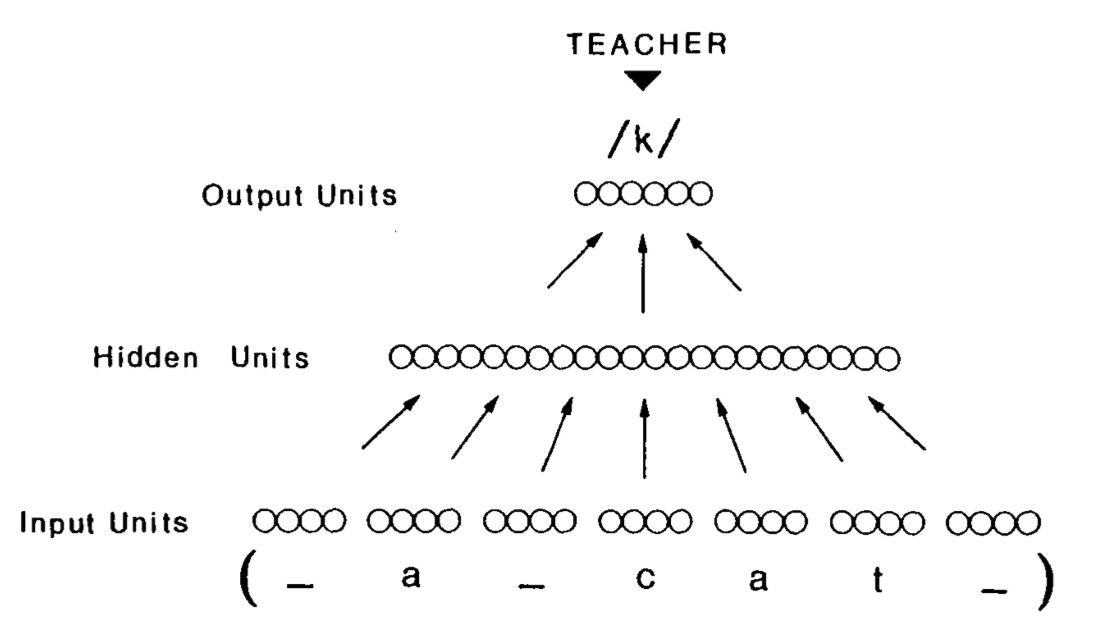
\includegraphics[width=12cm, height=8cm]{../out/images/recurrent-networks}
    \caption[recurrent networks]{recurrent networks}
    \label{fig: recurrent networks}
\end{figure}

For each of the seven input characters, a one-hot encoding is used with 29
units (including the 26 letters, plus punctuation and word boundaries) making a
total of 203 inputs.
There were 80 hidden units with sigmoidal transfer function, and 26 outputs
encoding 21 articulatory features plus stress and syllable boundaries.

NetTalk gained a lot of media attention at the time, partly because the output
was hooked up to a speech synthesiser.
In the early stages of training, it sounds a bit like a babbling baby.
When fully trained, it sounds reasonable, although somewhat robotic.

\frame{
    \frametitle{Embedded Video}
    \begin{center}
        \movie{\includegraphics[width=\textwidth]{}}{w4_language_processing/NETtalk Test.mp4}
    \end{center}
}

Critics have sometimes claimed that a decision tree could produce equally good
or better accuracy.
In any case, this kind of approach can only learn short-term dependencies, not
the medium or long-term dependencies that are required for some tasks.

\section{Simple Recurrent Network}\label{sec:simple-recurrent-network}

\begin{figure}[h]
    \centering
    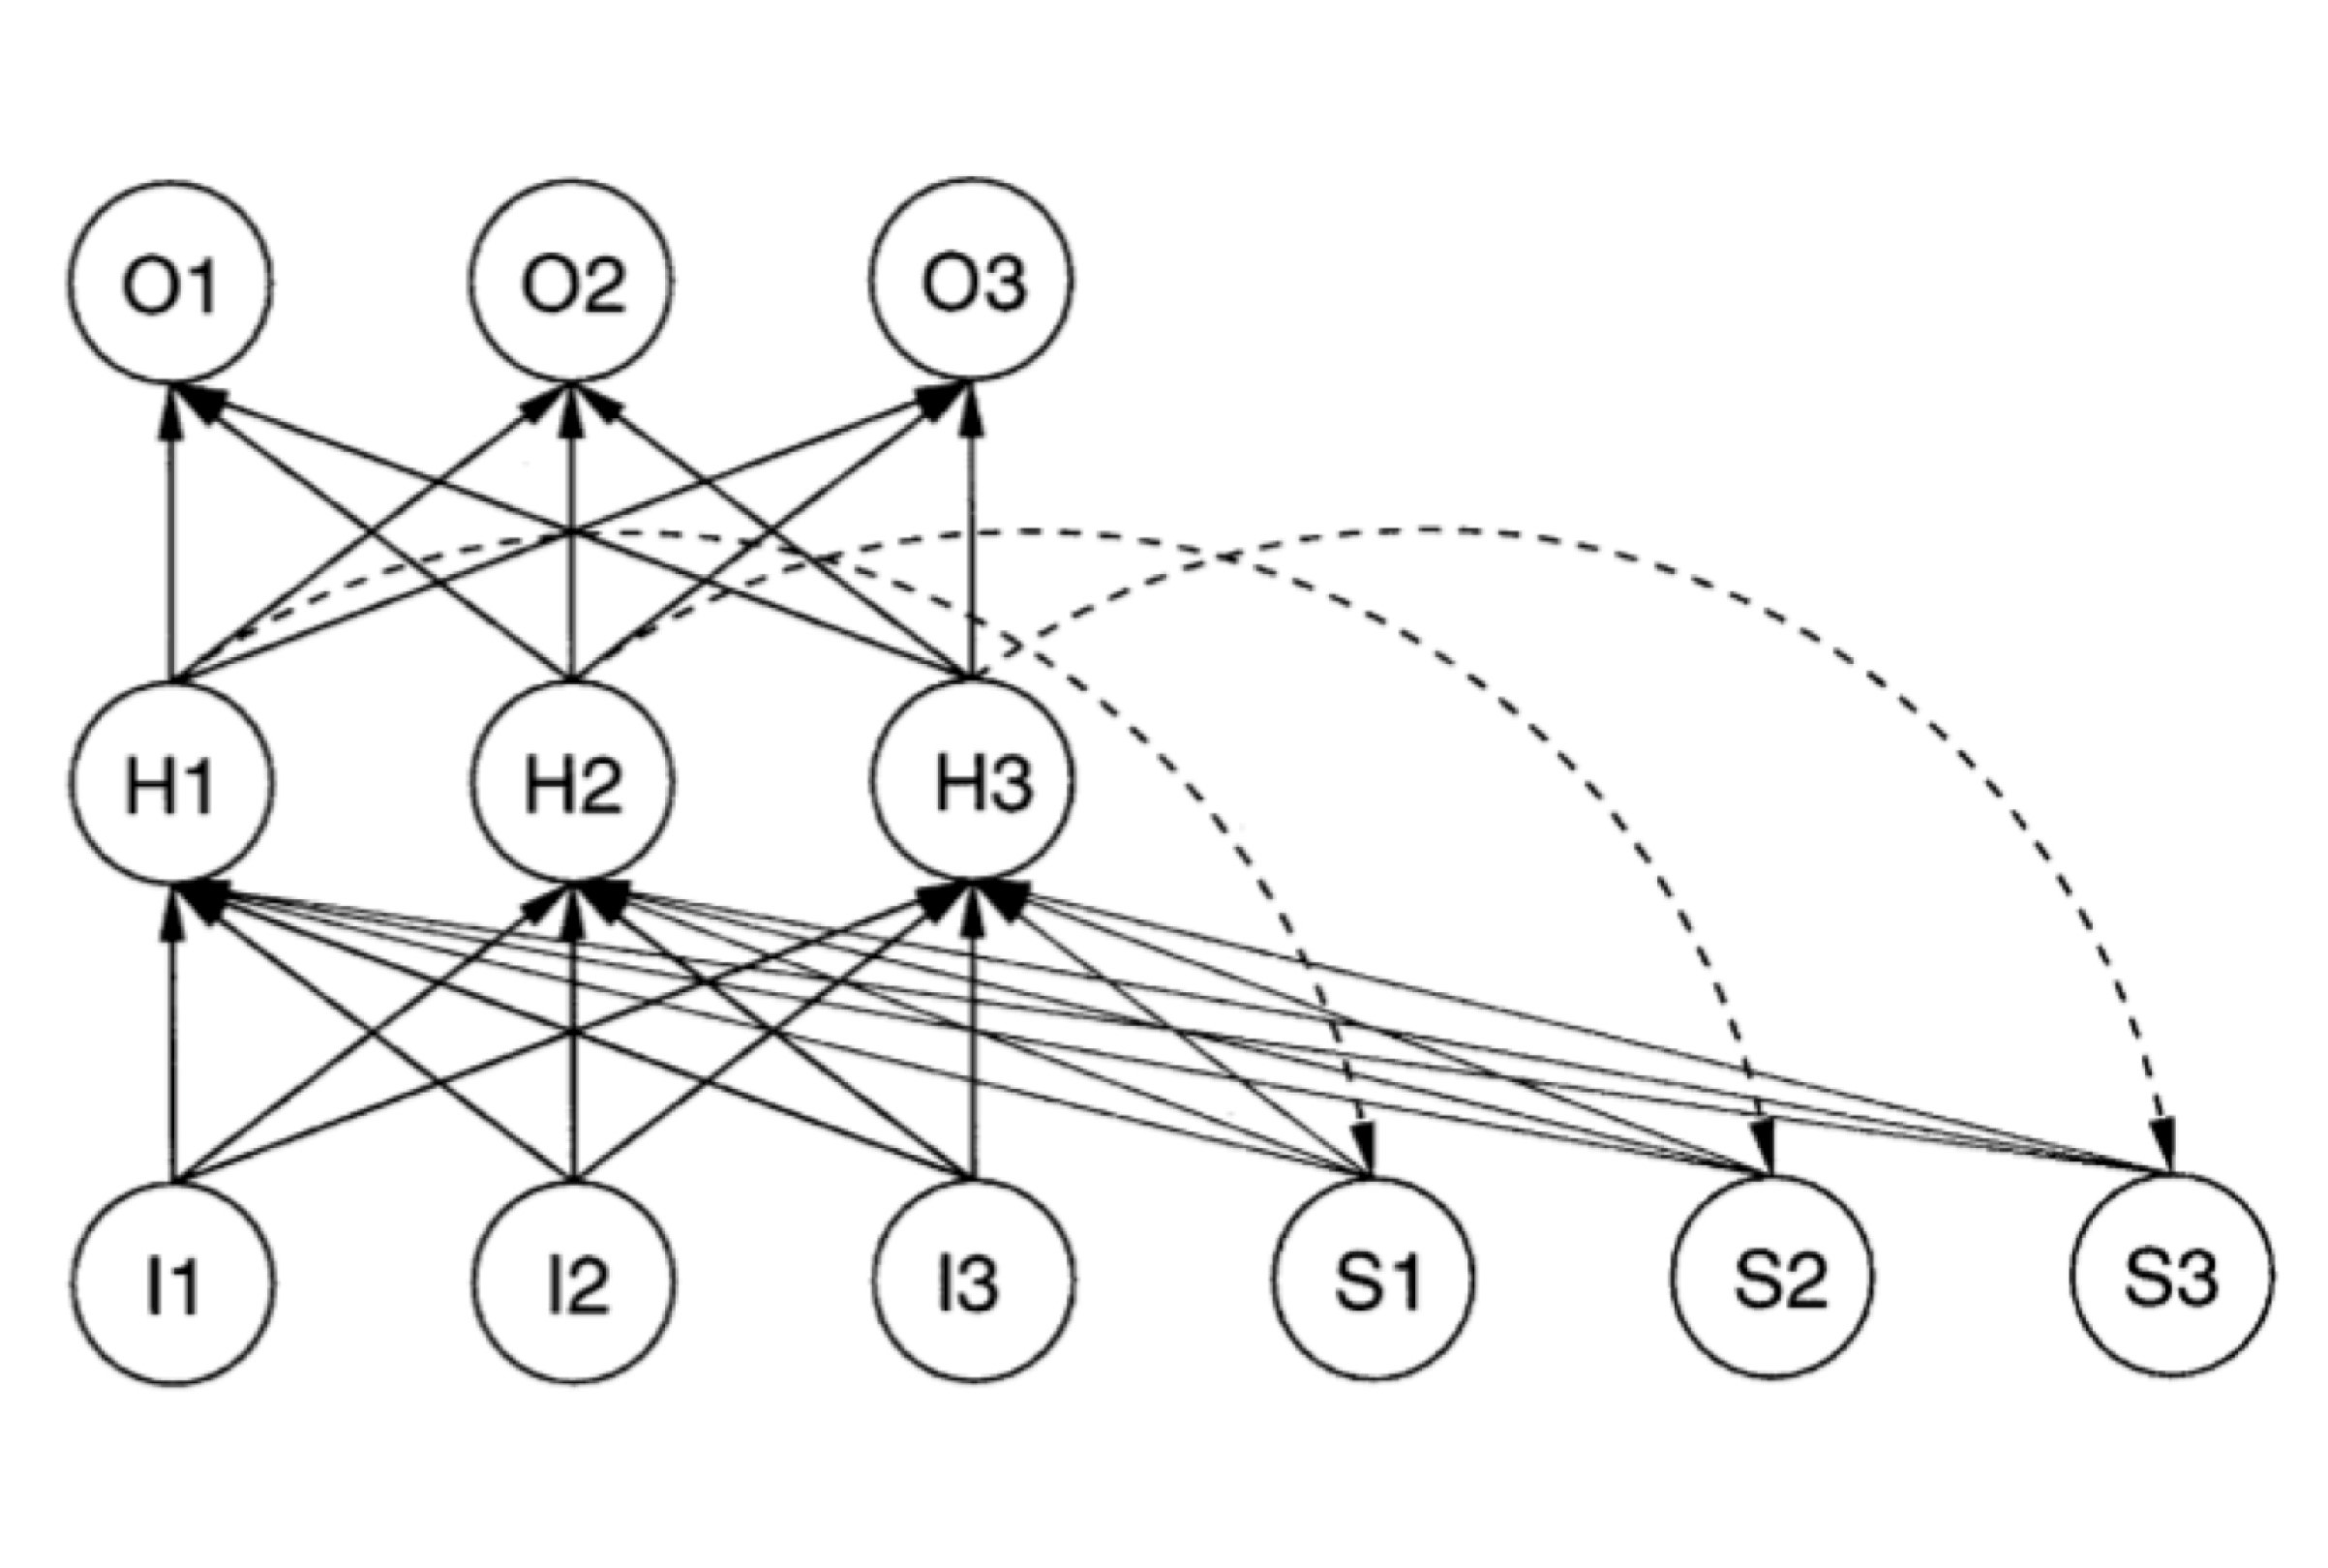
\includegraphics[width=8cm, height=7cm]{../out/images/simple-recurrent-network}
    \caption[simple recurrent network]{simple recurrent network}
    \label{fig: simple recurrent network}
\end{figure}

Simple Recurrent Networks (SRN) were introduced in Elman (1990).
A sequence of inputs are fed to the network one at a time.
At each timestep, the current activations in the hidden layer are copied to a
*context* layer.
The new activations for the hidden layer are then calculated from the current
input and the context layer.
Thus, the context layer is used to *remember* whatever information the network
requires in order to predict the correct output.

The basic SRN can be augmented with *shortcut* connections directly from input
to output, or connections from the output back to the hidden layer (sometimes
called “Jordan Networks”).

\section{Backpropagation Through Time}\label{sec:backpropagation-through-time}

For any given input sequence, we can *unroll* a recurrent architecture into an
equivalent feedforward architecture, with shared weights.
Applying backpropagation to the unrolled architecture is referred to as
**backpropagation through time**.
We can backpropagate just one timestep, or a fixed number of timesteps, or all
the way back to the beginning of the sequence.

\begin{figure}[h]
    \centering
    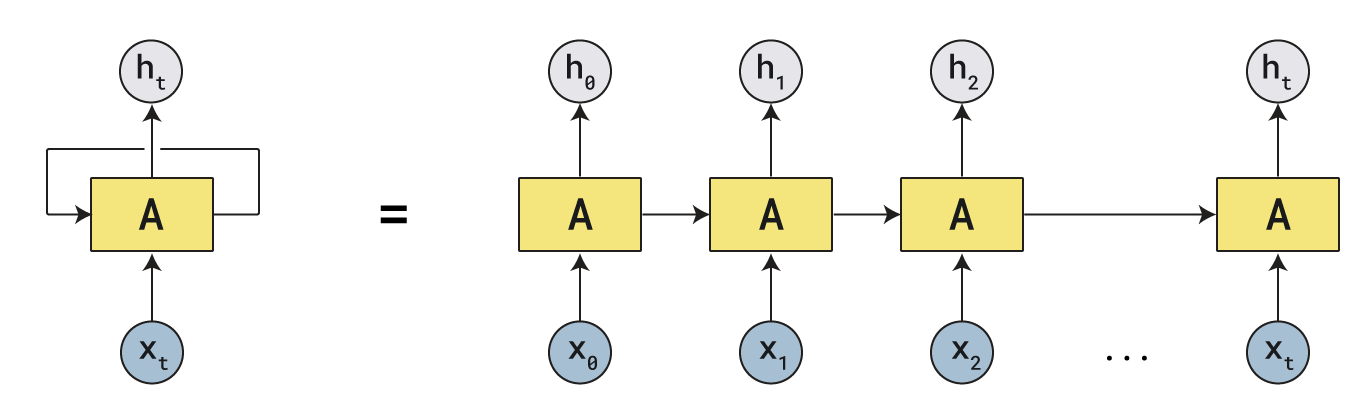
\includegraphics[width=12cm, height=8cm]{../out/images/back-propagation-through-time}
    \caption[back propagation through time]{back propagation through time}
    \label{fig: back propagation through time}
\end{figure}

\href{http://colah.github.io/posts/2015-08-Understanding-LSTMs/}{Understanding LSTMs}

insert video

\section{Recognizers and Predictors}\label{sec:recognizers-and-predictors}
The basic SRN can be augmented with *shortcut* connections directly from input
to output, or connections from the output back to the hidden layer (sometimes
called “Jordan Networks”).
Another architecture which has been explored for binary sequences is the Second
Order Network or Gated Network, where the input symbol ($$0$ or $1$$) is used
to choose between two sets of weights $W_0$ and $W_1$.
The weights $W0$, $W_1$ and $P$ and the initial state $x_0$ can all be trained
by backpropagation through time.

\begin{figure}[h]
    \centering
    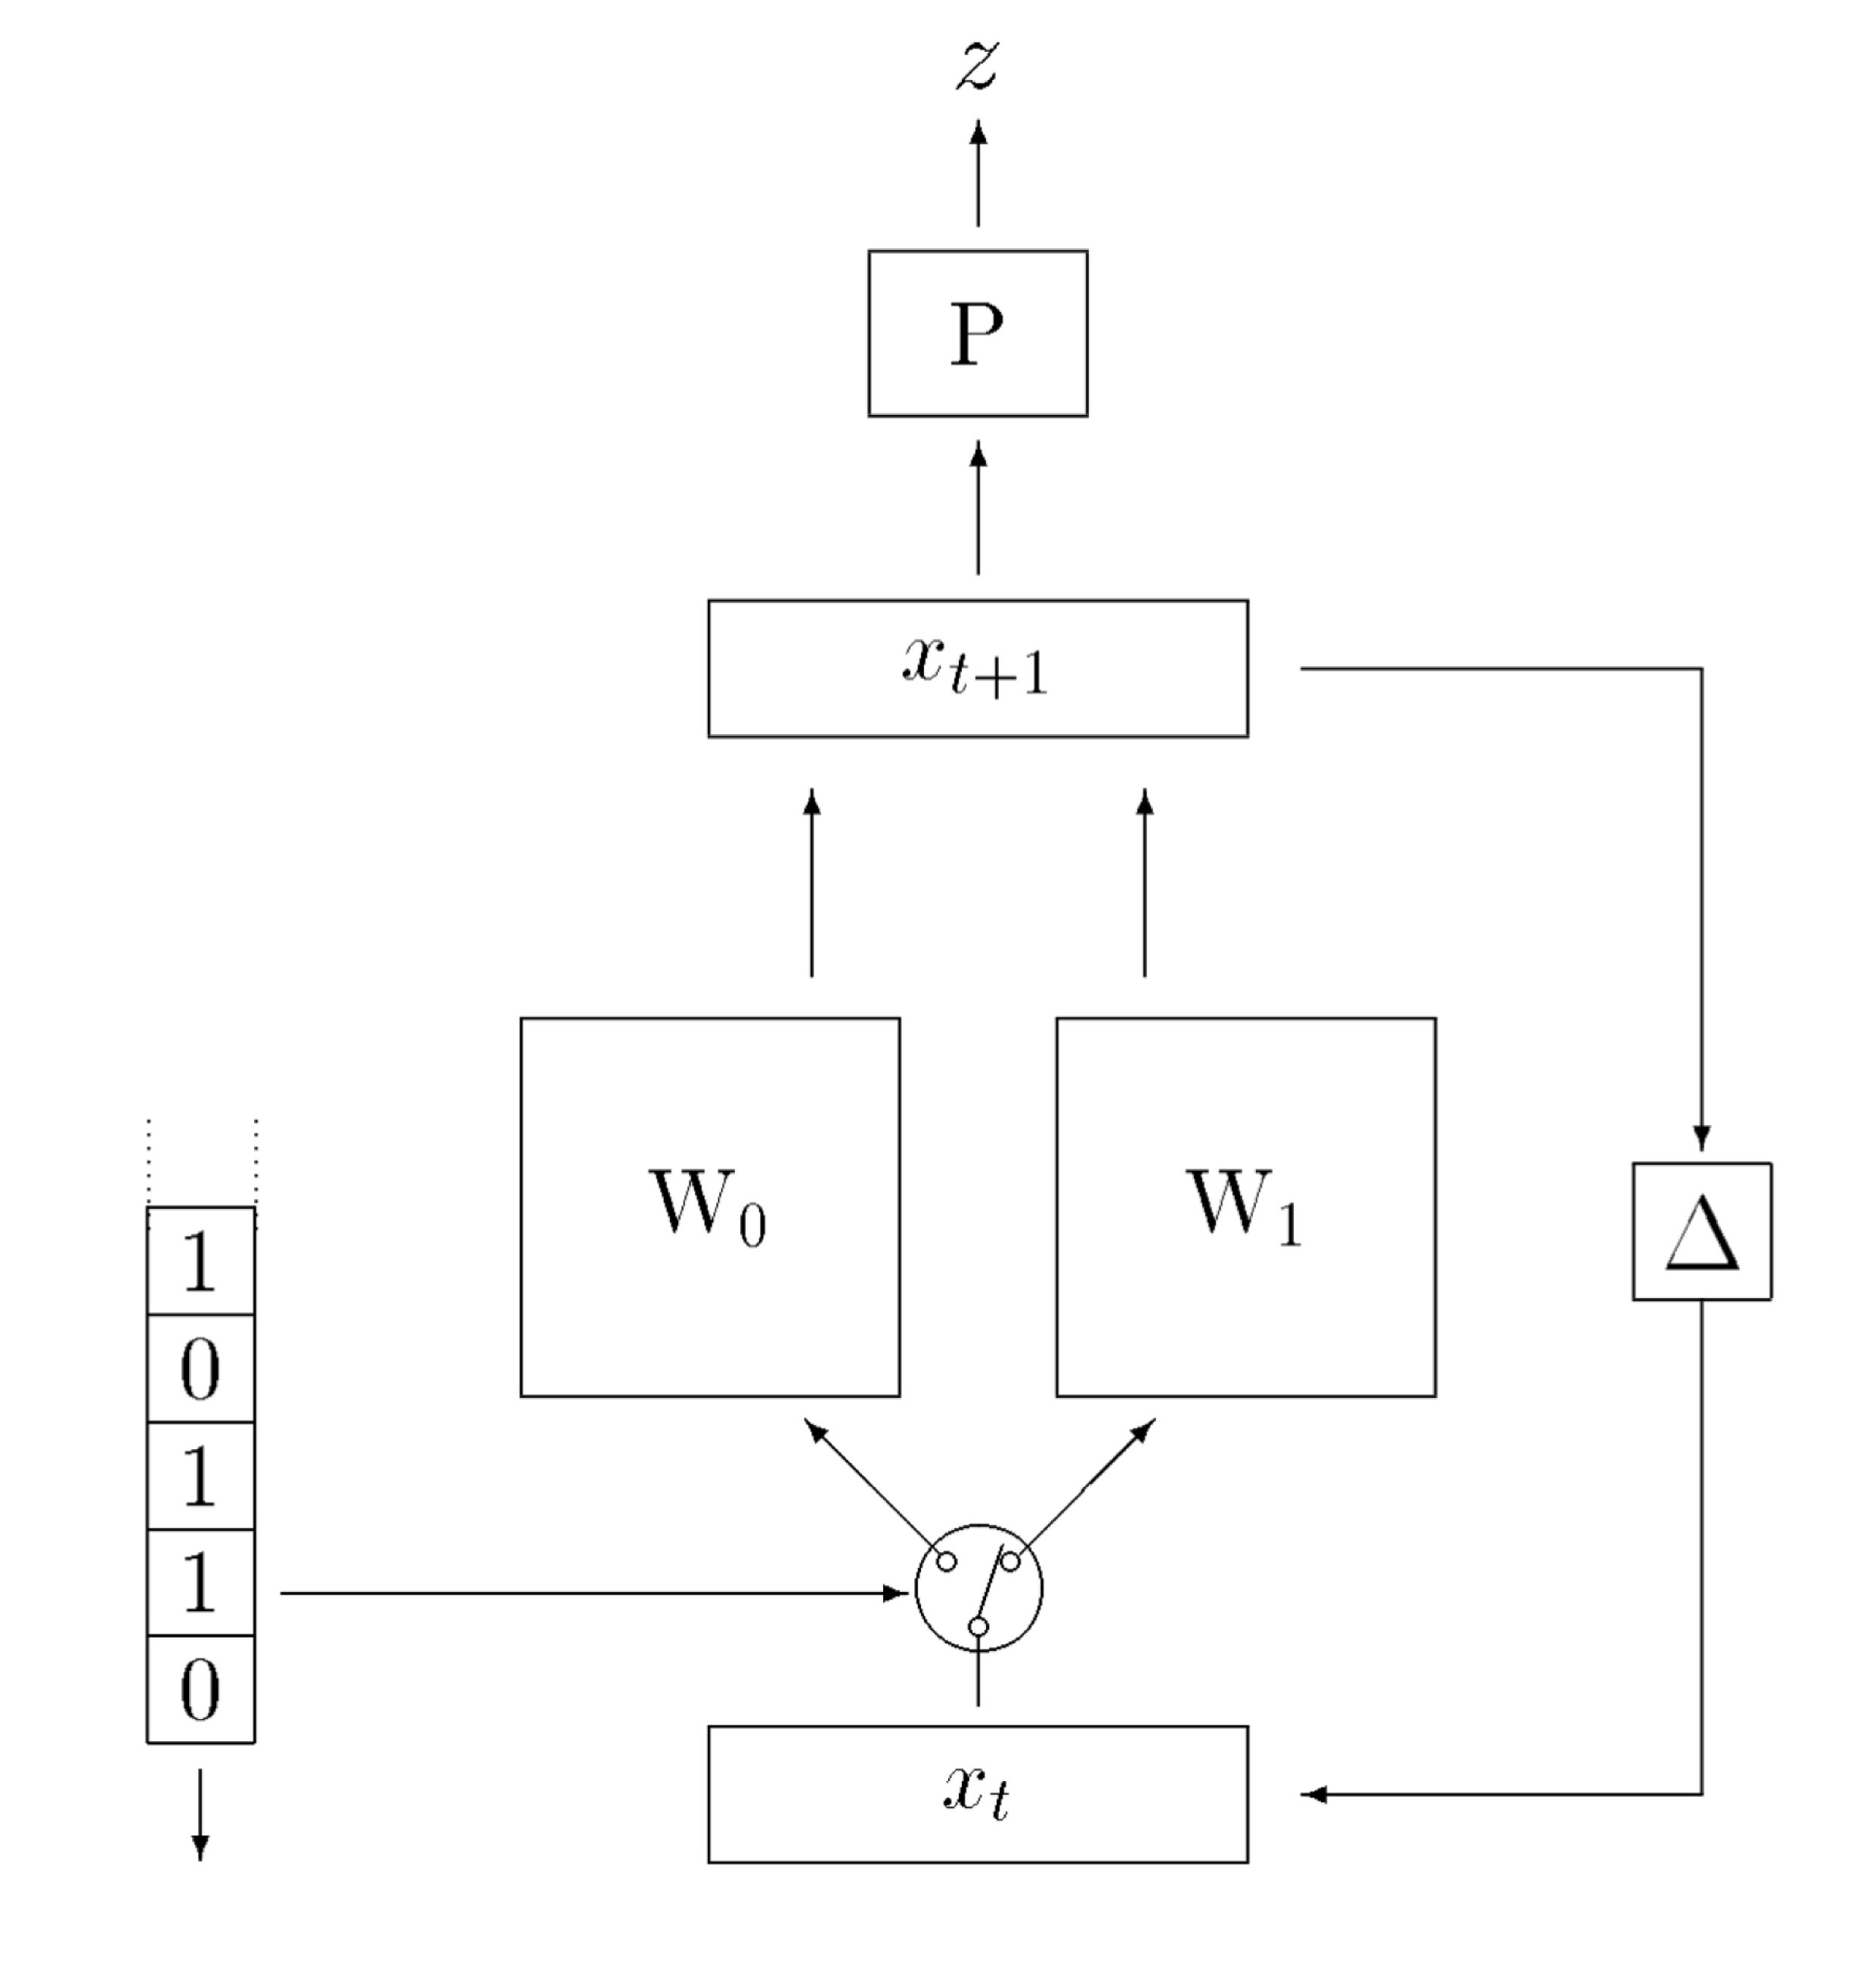
\includegraphics[width=12cm, height=8cm]{../out/images/recognisers_and_ports}
    \caption{recognisers and ports}
    \label{fig: recognisers and ports}
\end{figure}

\section{Dynamical Recognizers}\label{sec:dynamical-recognizers}

    One common sequence processing task is Formal Language Recognition.
The network scans a sequence of characters one at a time, and must then output
either $1$ or $0$, in order to classify the sequence as Accept or Reject, respectively.
Consider, for example, this set of training data:

\begin{center}
\begin{tabular}{ |c|c|c| }
 \hline
 Accept & Reject \\
 1 & 0 \\
 11 & 10 \\
 111 & 01 \\
 1111 & 00 \\
 11111 & 011 \\
 111111 & 110 \\
 1111111 & 11111110\\
 11111111 & 10111111\\
 \hline
\end{tabular}
\end{center}

The natural generalisation from these data is to classify strings consisting
entirely of $1$s as Accept and any string containing 000 as Reject.
This diagram shows the result of training a Second Order Network on these data.
The cross indicates the initial state while the dots indicate all the hidden
states which occur while the network is processing a set of randomly generated
test strings.
The dividing line shows the boundary between final states for which the string
is classified as Accept, and those for which it is classified as Reject.

\begin{figure}[h]
    \centering
    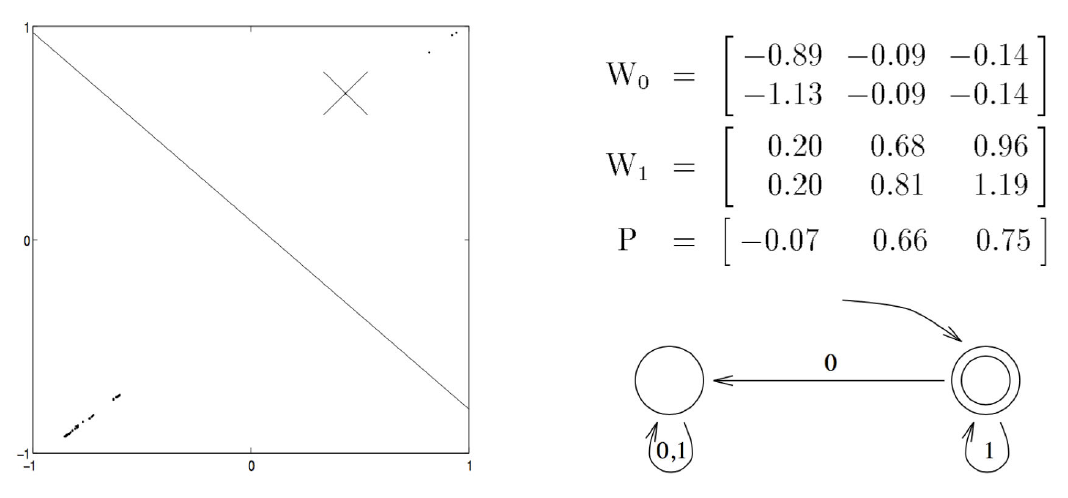
\includegraphics[width=12cm, height=8cm]{../out/images/dynamic-recognisers}
    \caption{}
    \label{fig: dynamic recognisers}
\end{figure}

In some cases, we can use analytical tools to extract a finite state machine
which exactly mimics the behaviour of the network, as shown on the right for
this example (Blair and Pollack, 1997).
Each cluster of hidden unit states is converted into a single state, the
transitions between clusters are converted into arrows, and the initial state
is indicated by an arrow with no origin.
The state(s) on the Accept side of the dividing line are indicated by a double
circle;
those on the Reject side by a single circle.

Here is another example, where the network learns to Reject any string with
three consecutive $0$s and Accept everything else.

\begin{center}
\begin{tabular}{ |c|c|c| }
 \hline
 cell1 & cell2 & cell3 \\
 cell4 & cell5 & cell6 \\
 cell7 & cell8 & cell9 \\
 \hline
\end{tabular}
\end{center}

\begin{figure}[h]
    \centering
    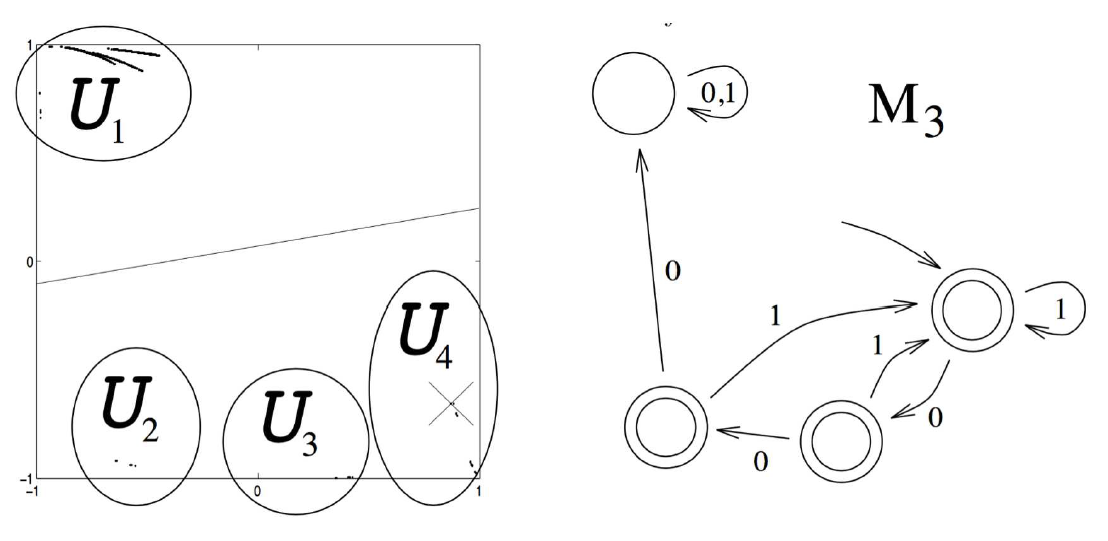
\includegraphics[width=12cm, height=10cm]{../out/images/dynamic-recognisers-2}
    \caption{dynamic recognisers 2}
    \label{fig: dynamic recognisers 2}
\end{figure}

In some cases, we can use analytical tools to extract a finite state machine
which exactly mimics the behaviour of the network, as shown on the right for
this example (Blair and Pollack, 1997).
Each cluster of hidden unit states is converted into a single state, the
transitions between clusters are converted into arrows, and the initial state
is indicated by an arrow with no origin.
The state(s) on the Accept side of the dividing line are indicated by a double
circle;
those on the Reject side by a single circle.

Here is another example, where the network learns to Reject any string with
three consecutive $0$s and Accept everything else.

\begin{center}
\begin{tabular}{ |c|c|c| }
 \hline
 Accept & Reject \\
 1 & 000 \\
 0 & 11000 \\
 10 & 0001 \\
 01 & 000000000 \\
 00 & 11111000011 \\
 100100 & 11111000011 \\
 001111110100 & 1101010000010111 \\
 0100100100 & 1010010001 \\
 0100100100 & 0000 \\
 11100 & 00000 \\
 \hline
\end{tabular}
\end{center}

\begin{figure}[h]
    \centering
    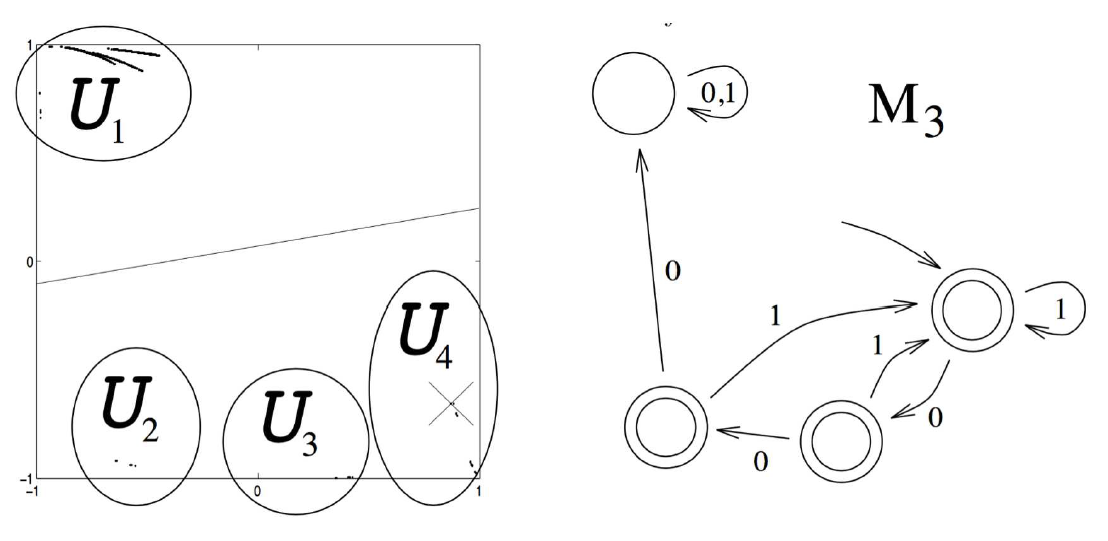
\includegraphics[width=12cm, height=8cm]{../out/images/dynamic-recognisers-4}
    \caption[dynamic recognisers 4]{dynamic recognisers 4}
    \label{fig: dynamic recognisers 4}
\end{figure}


\section{Non-Regular languages}\label{sec:non-regular-languages}
Languages which can be characterized by a finite state machine are called
Regular languages.
One simple example of a non-Regular language is $a^n b^n$ which means that
every sequence of consecutive $a$s must be followed by an equal number of
consecutive $b$s −-− for example:

abaabbabaaabbbaaaabbbbabaabbaaaaabbbbb. . .

A SRN with 2 inputs, 2 hidden nodes and 2 outputs can be trained to predict the
$a^n b^n$ language (Wiles and Elman, 1995).
In this case, the network must scan a sequence of input characters one at a
time, and try at each step to predict the next character in the sequence.
In some cases, the prediction is probabilistic.
For the $a^n b^n$ task, the first $b$ is not predictable, but subsequent $b$
and the initial $a$ in the next subsequence are predictable.

    \begin{figure}[h]
    \centering
    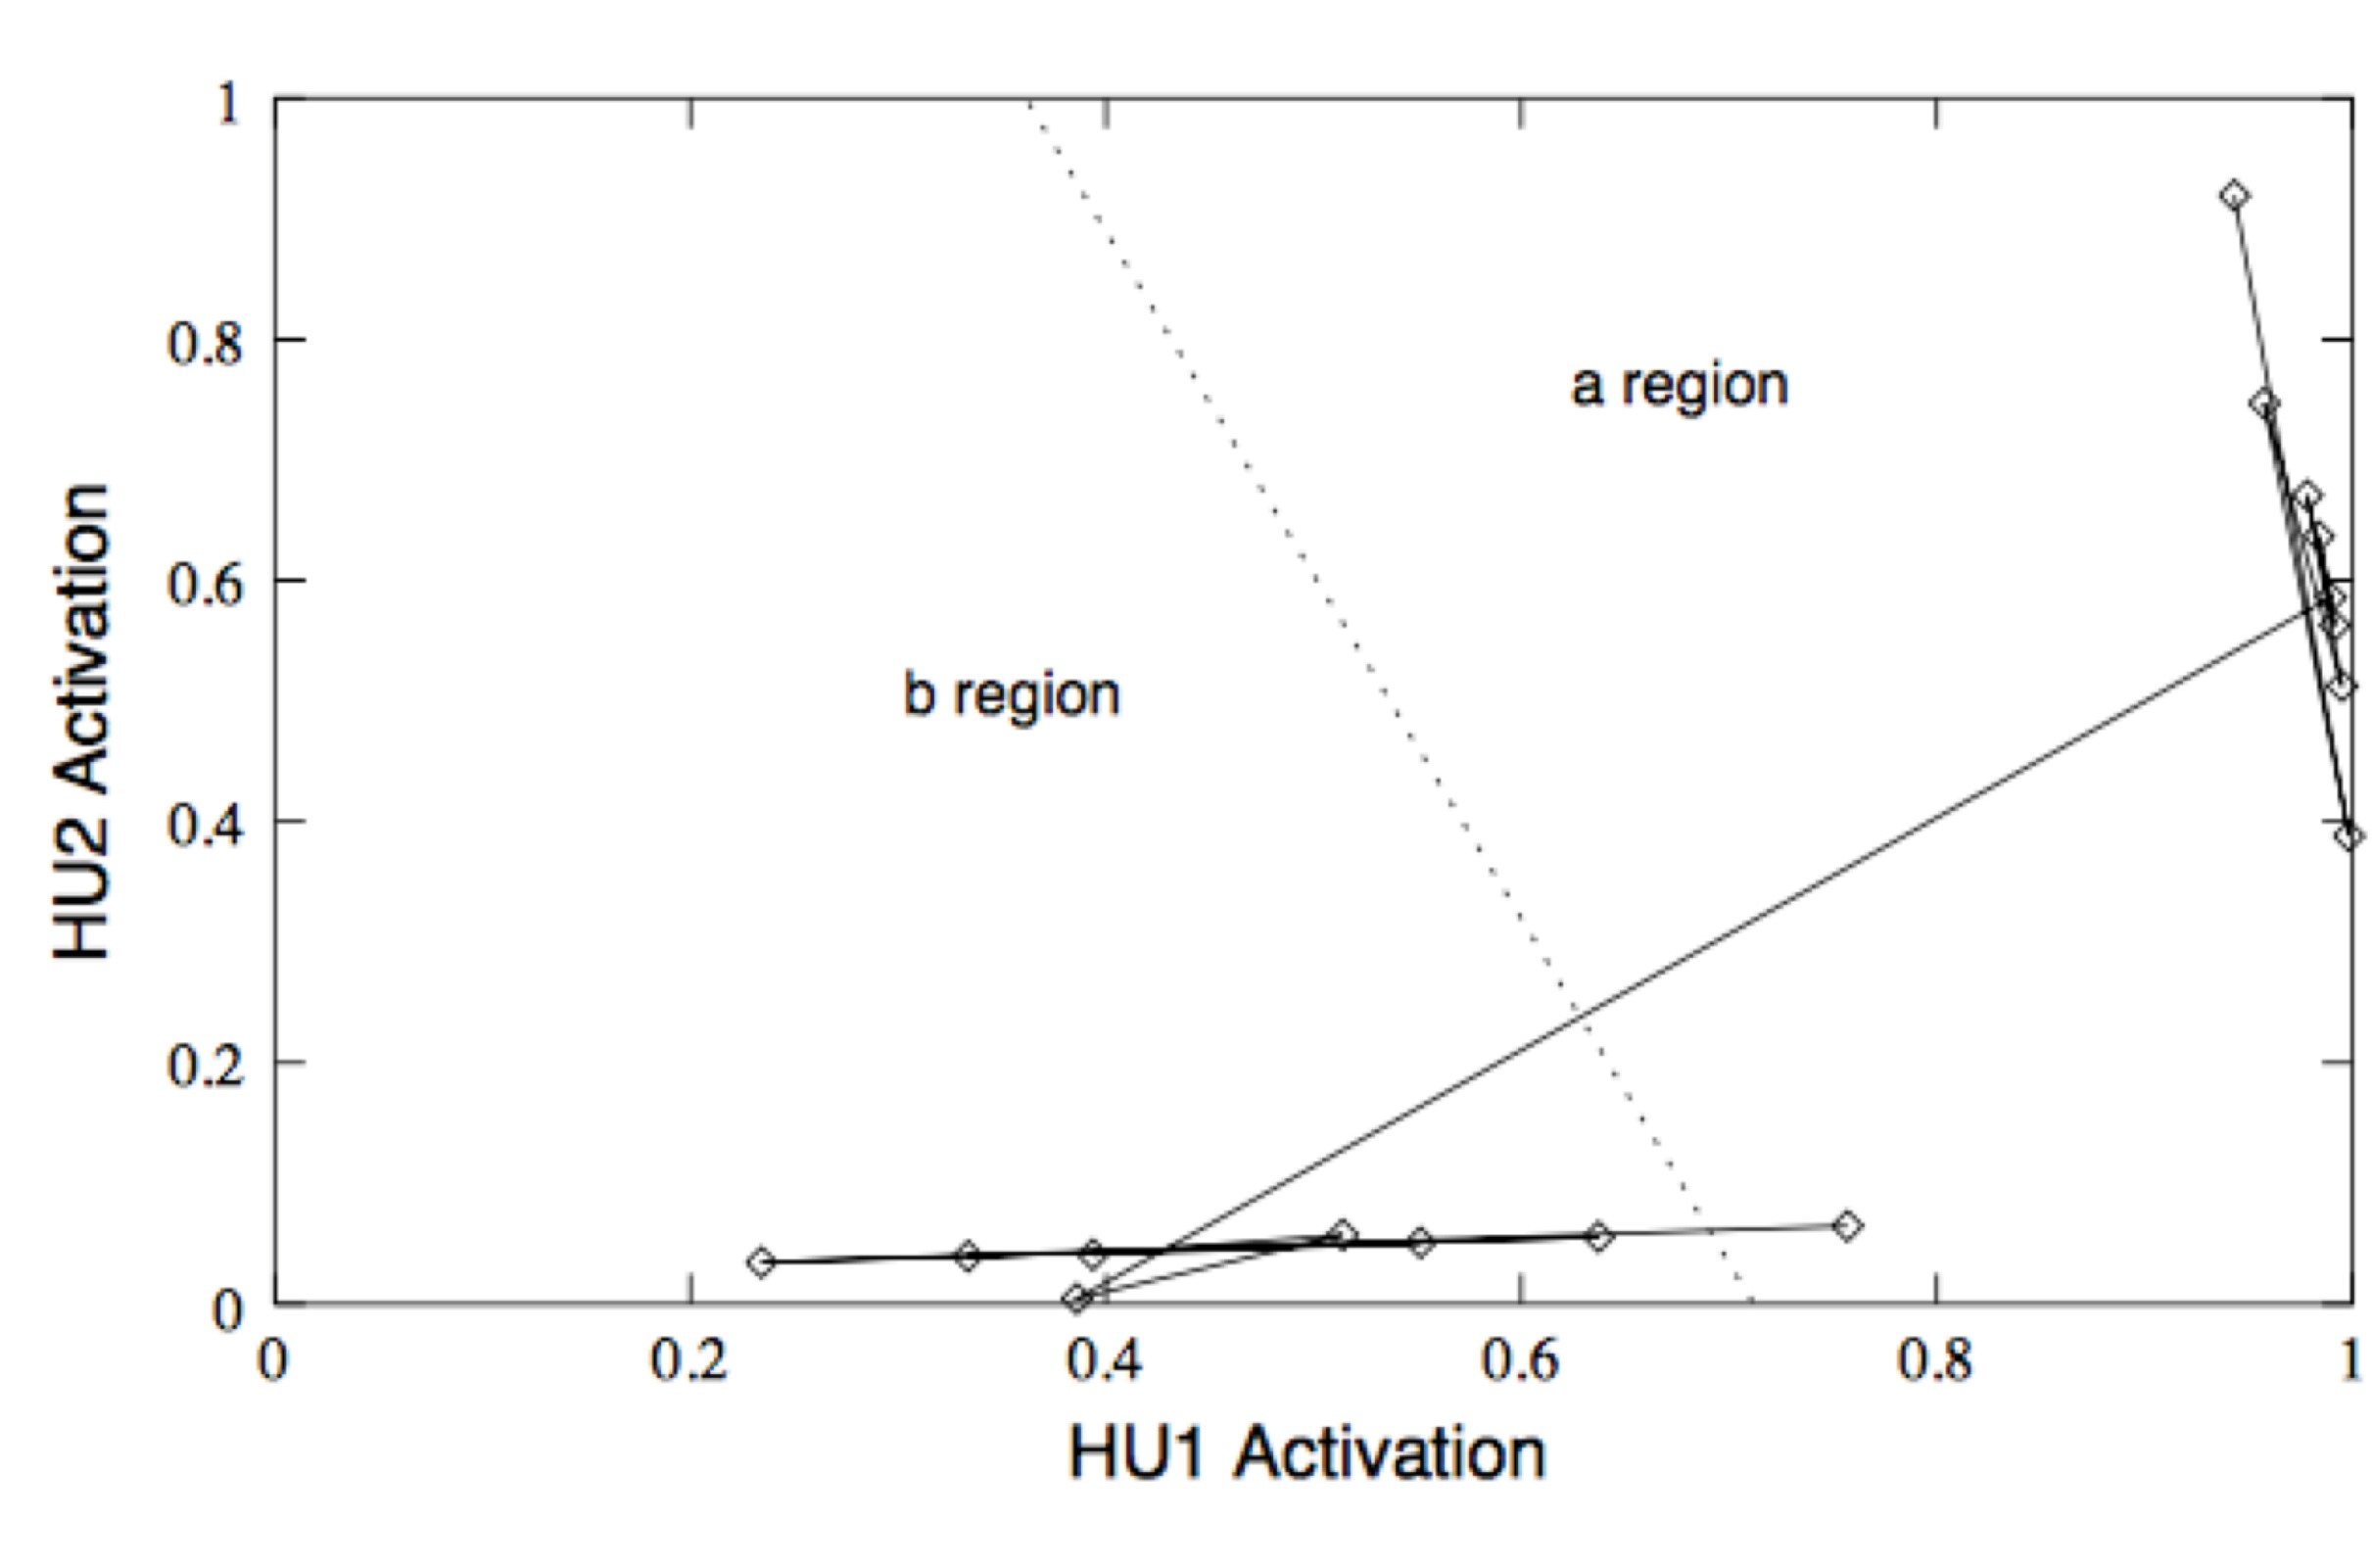
\includegraphics[width=12cm, height=8cm]{../out/images/non-regular-languages}
    \caption[non-regular languages]{non-regular languages}
    \label{fig: non-regular languages}
    \end{figure}

The network does not implement a Finite State Machine but instead makes use of
two fixed points in activation space ––– one attracting, the other repelling
(Wiles and Elman, 1995).
The network effectively *counts up* the $a$s as it oscillates towards the
attractive fixed point and then counts down the same number of bbb's as it
oscillates away from the repelling fixed point.
When the recurrent mapping is linearised at the two fixed points we find that
the two major eigenvalues are nearly reciprocal to each other.
Interestingly, networks trained only up to $a^{10} b^{10}$ can often generalise
up to $a^{12}b^{12}$.

Training the weights by evolution is more stable than by backpropagation.
Networks trained by evolution sometimes exhibit monotonic rather than
oscillating trajectories.

\begin{figure}[h]
    \centering
    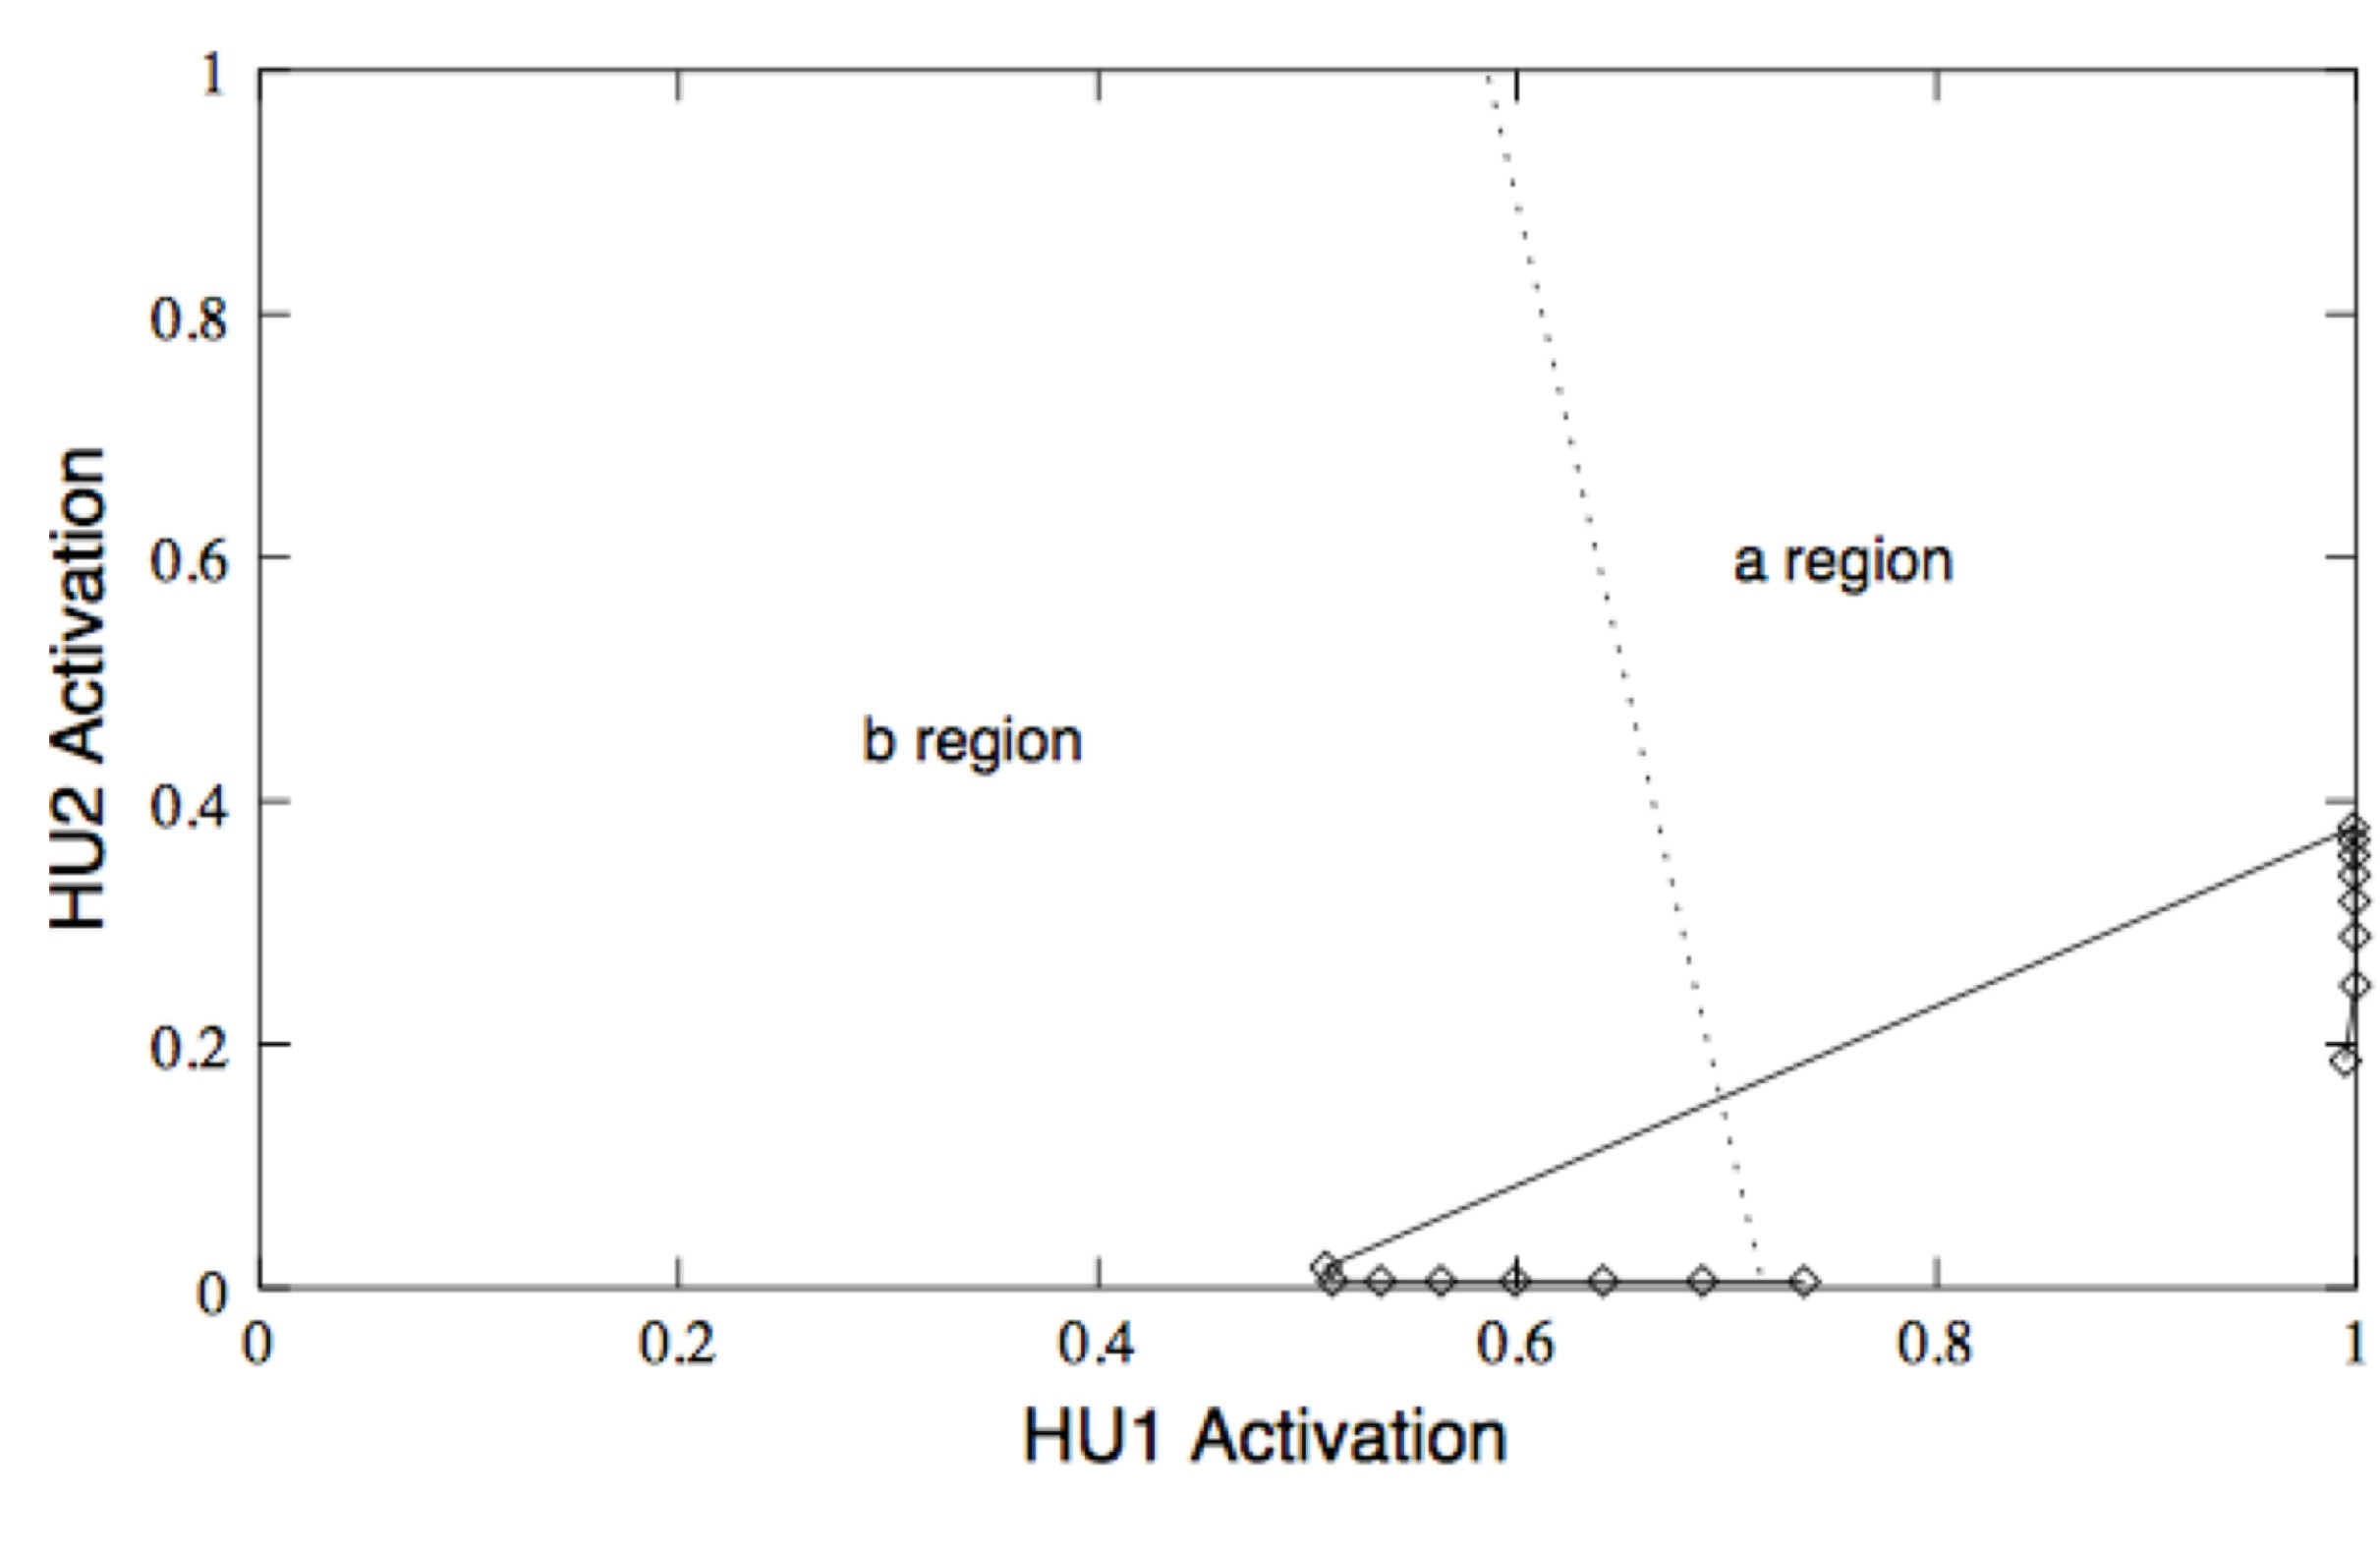
\includegraphics[width=12cm, height=8cm]{../out/images/non-regular-languages-2}
    \caption[non-regular languages 2]{non-regular languages 2}
    \label{fig: non-regular languages 2}
\end{figure}

\section{Counting by spiralling}\label{sec:counting-by-spiralling}
SRN's can also be trained to recognise the balanced bracket language, treating
$a$ as open bracket and bbb as close bracket (Boden, 2003).
In this case, the eigenvalues of the linearised mapping at the fixed points are
complex numbers, and the network counts up the $a$s by spiralling inwards
towards a fixed point and counts down the $b$s by spiralling outwards.

\begin{figure}[Hh]
    \centering
    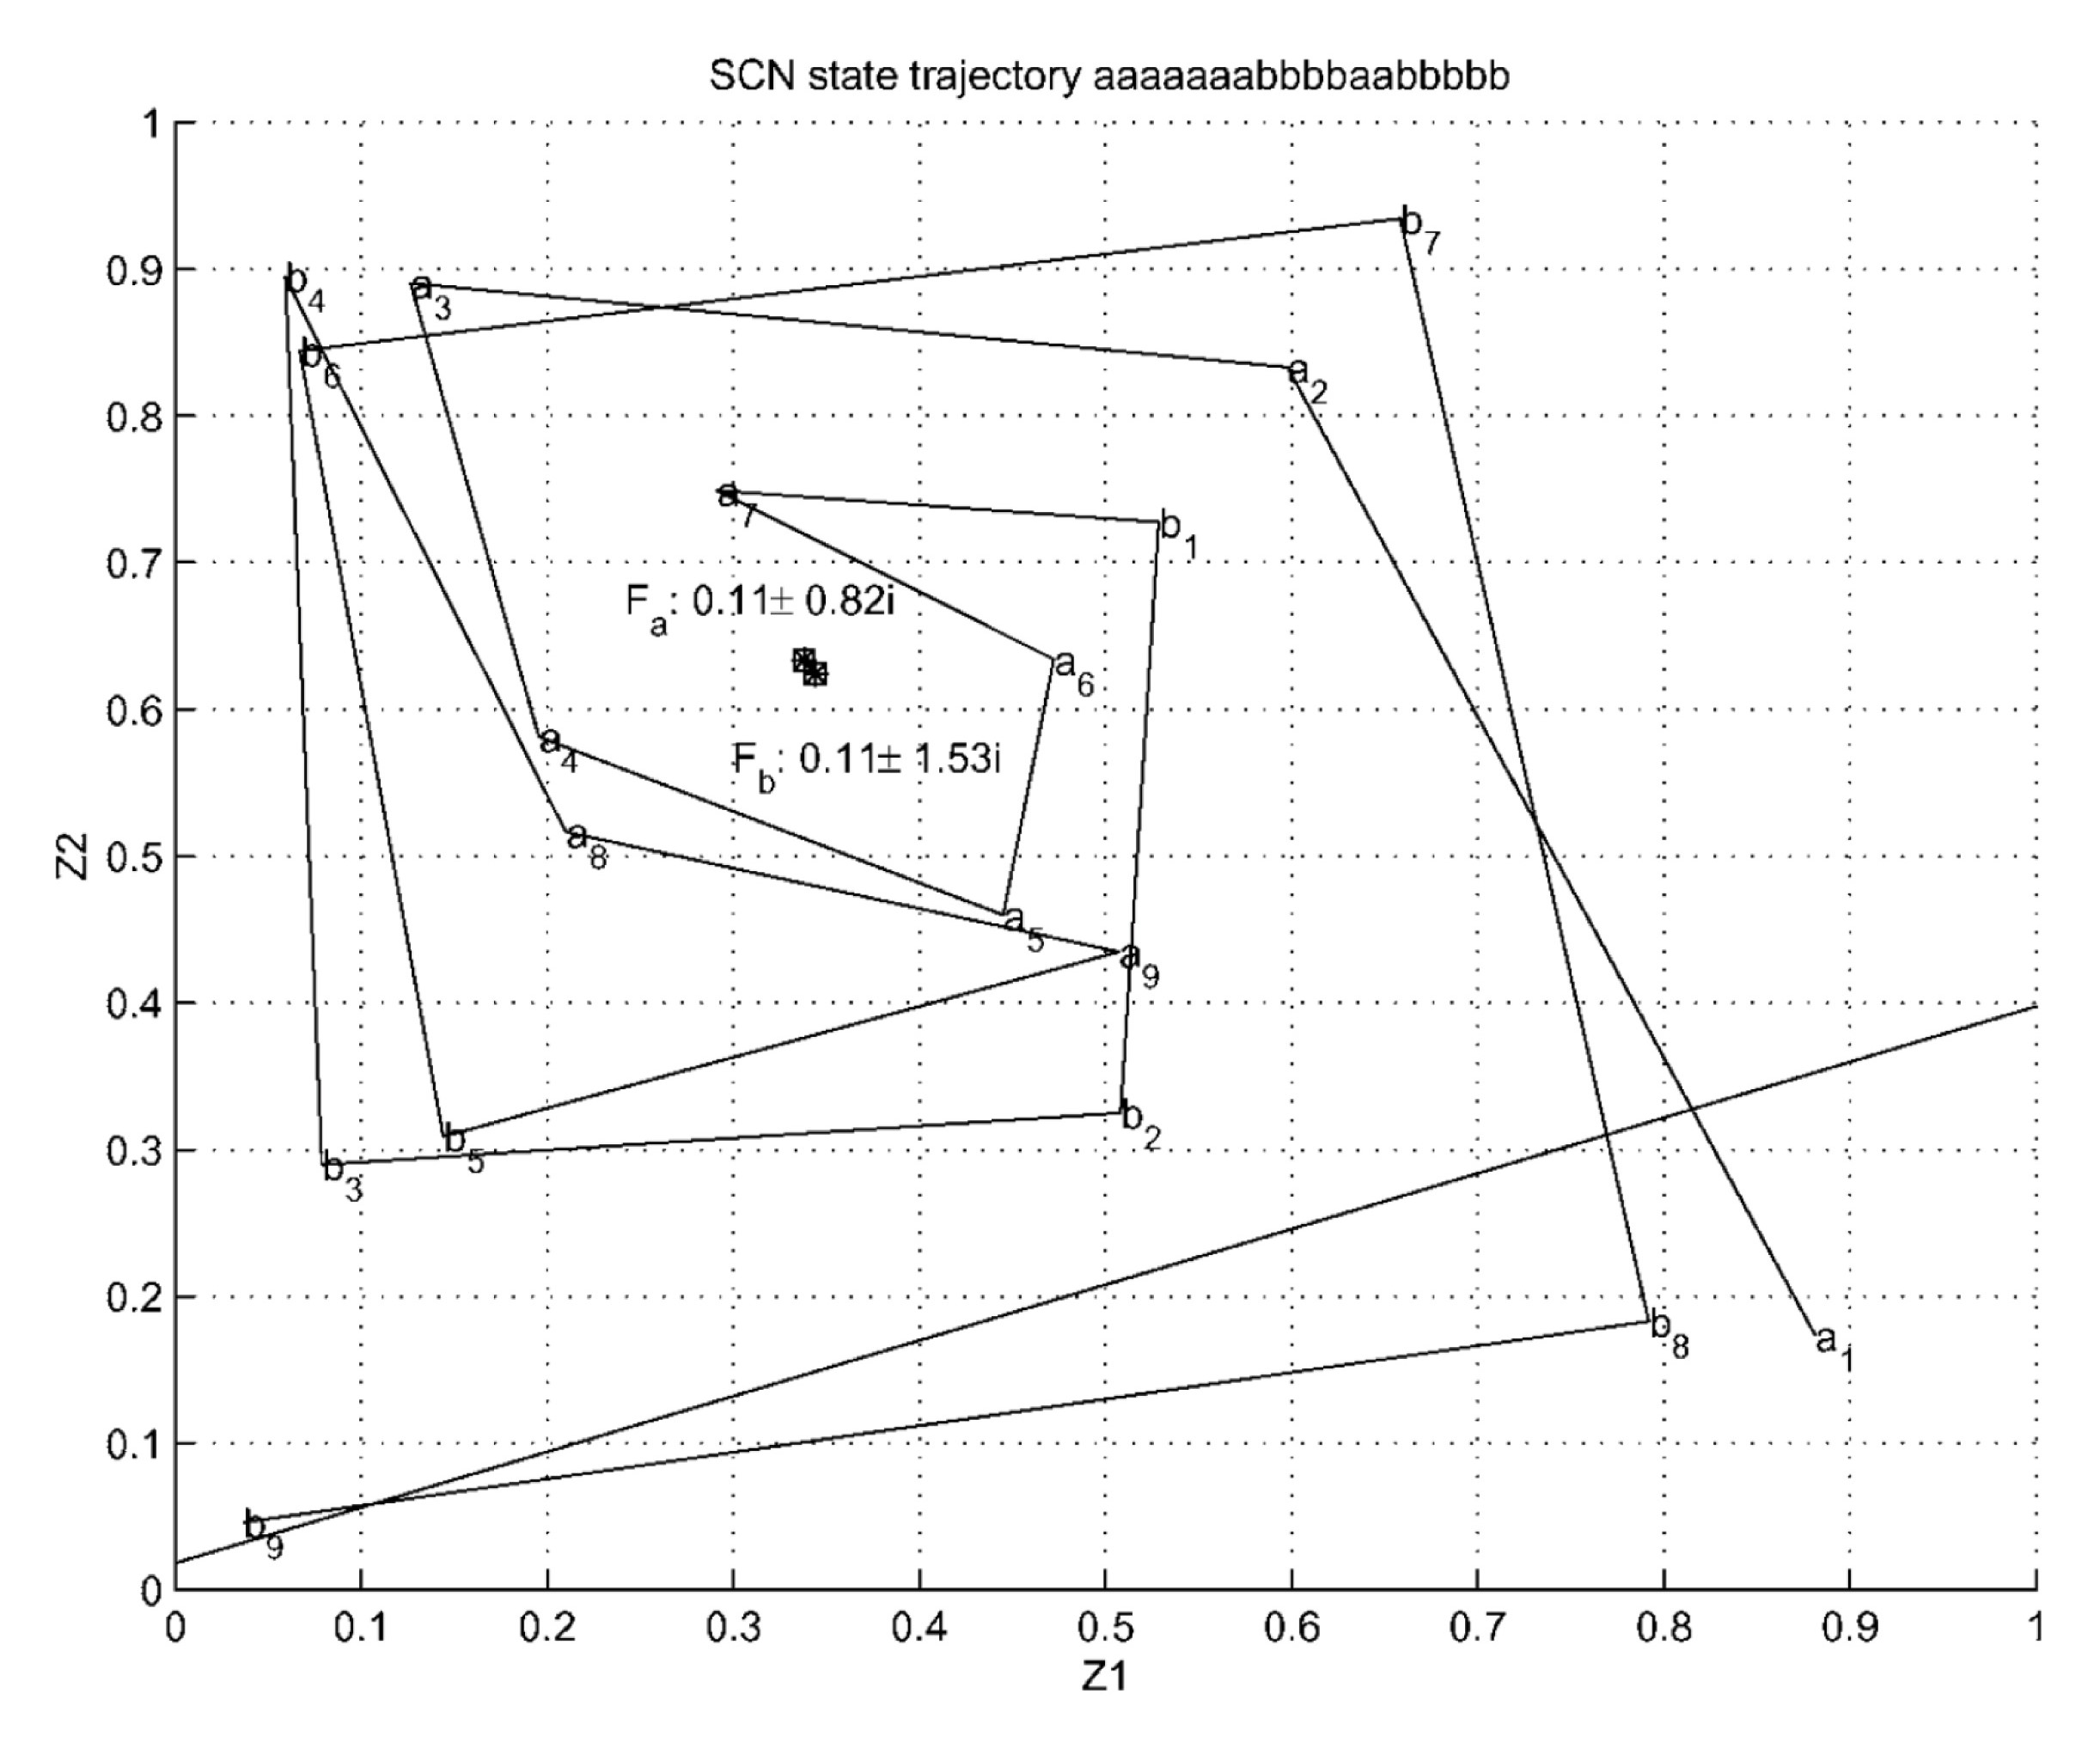
\includegraphics[width=12cm, height=8cm]{../out/images/counting-by-spiralling}
    \caption[counting by spiralling]{counting by spiralling}
    \label{fig: counting by spiralling}
\end{figure}

\section{Hidden Uni Dynamics for $a^n b^n c^n$}\label{sec:hidden-uni-dynamics-for-$a^n-b^n-c^n$}

An SRN with three inputs, three hidden units and three outputs can be used to learn the language $a^n b^n c^n$ which is classified as Mildly Context Sensitive (Chalup, 2003).
The network counts down in one direction while simultaneously counting up in another direction, thus producing a star-shaped pattern.

\begin{figure}[h]
    \centering
    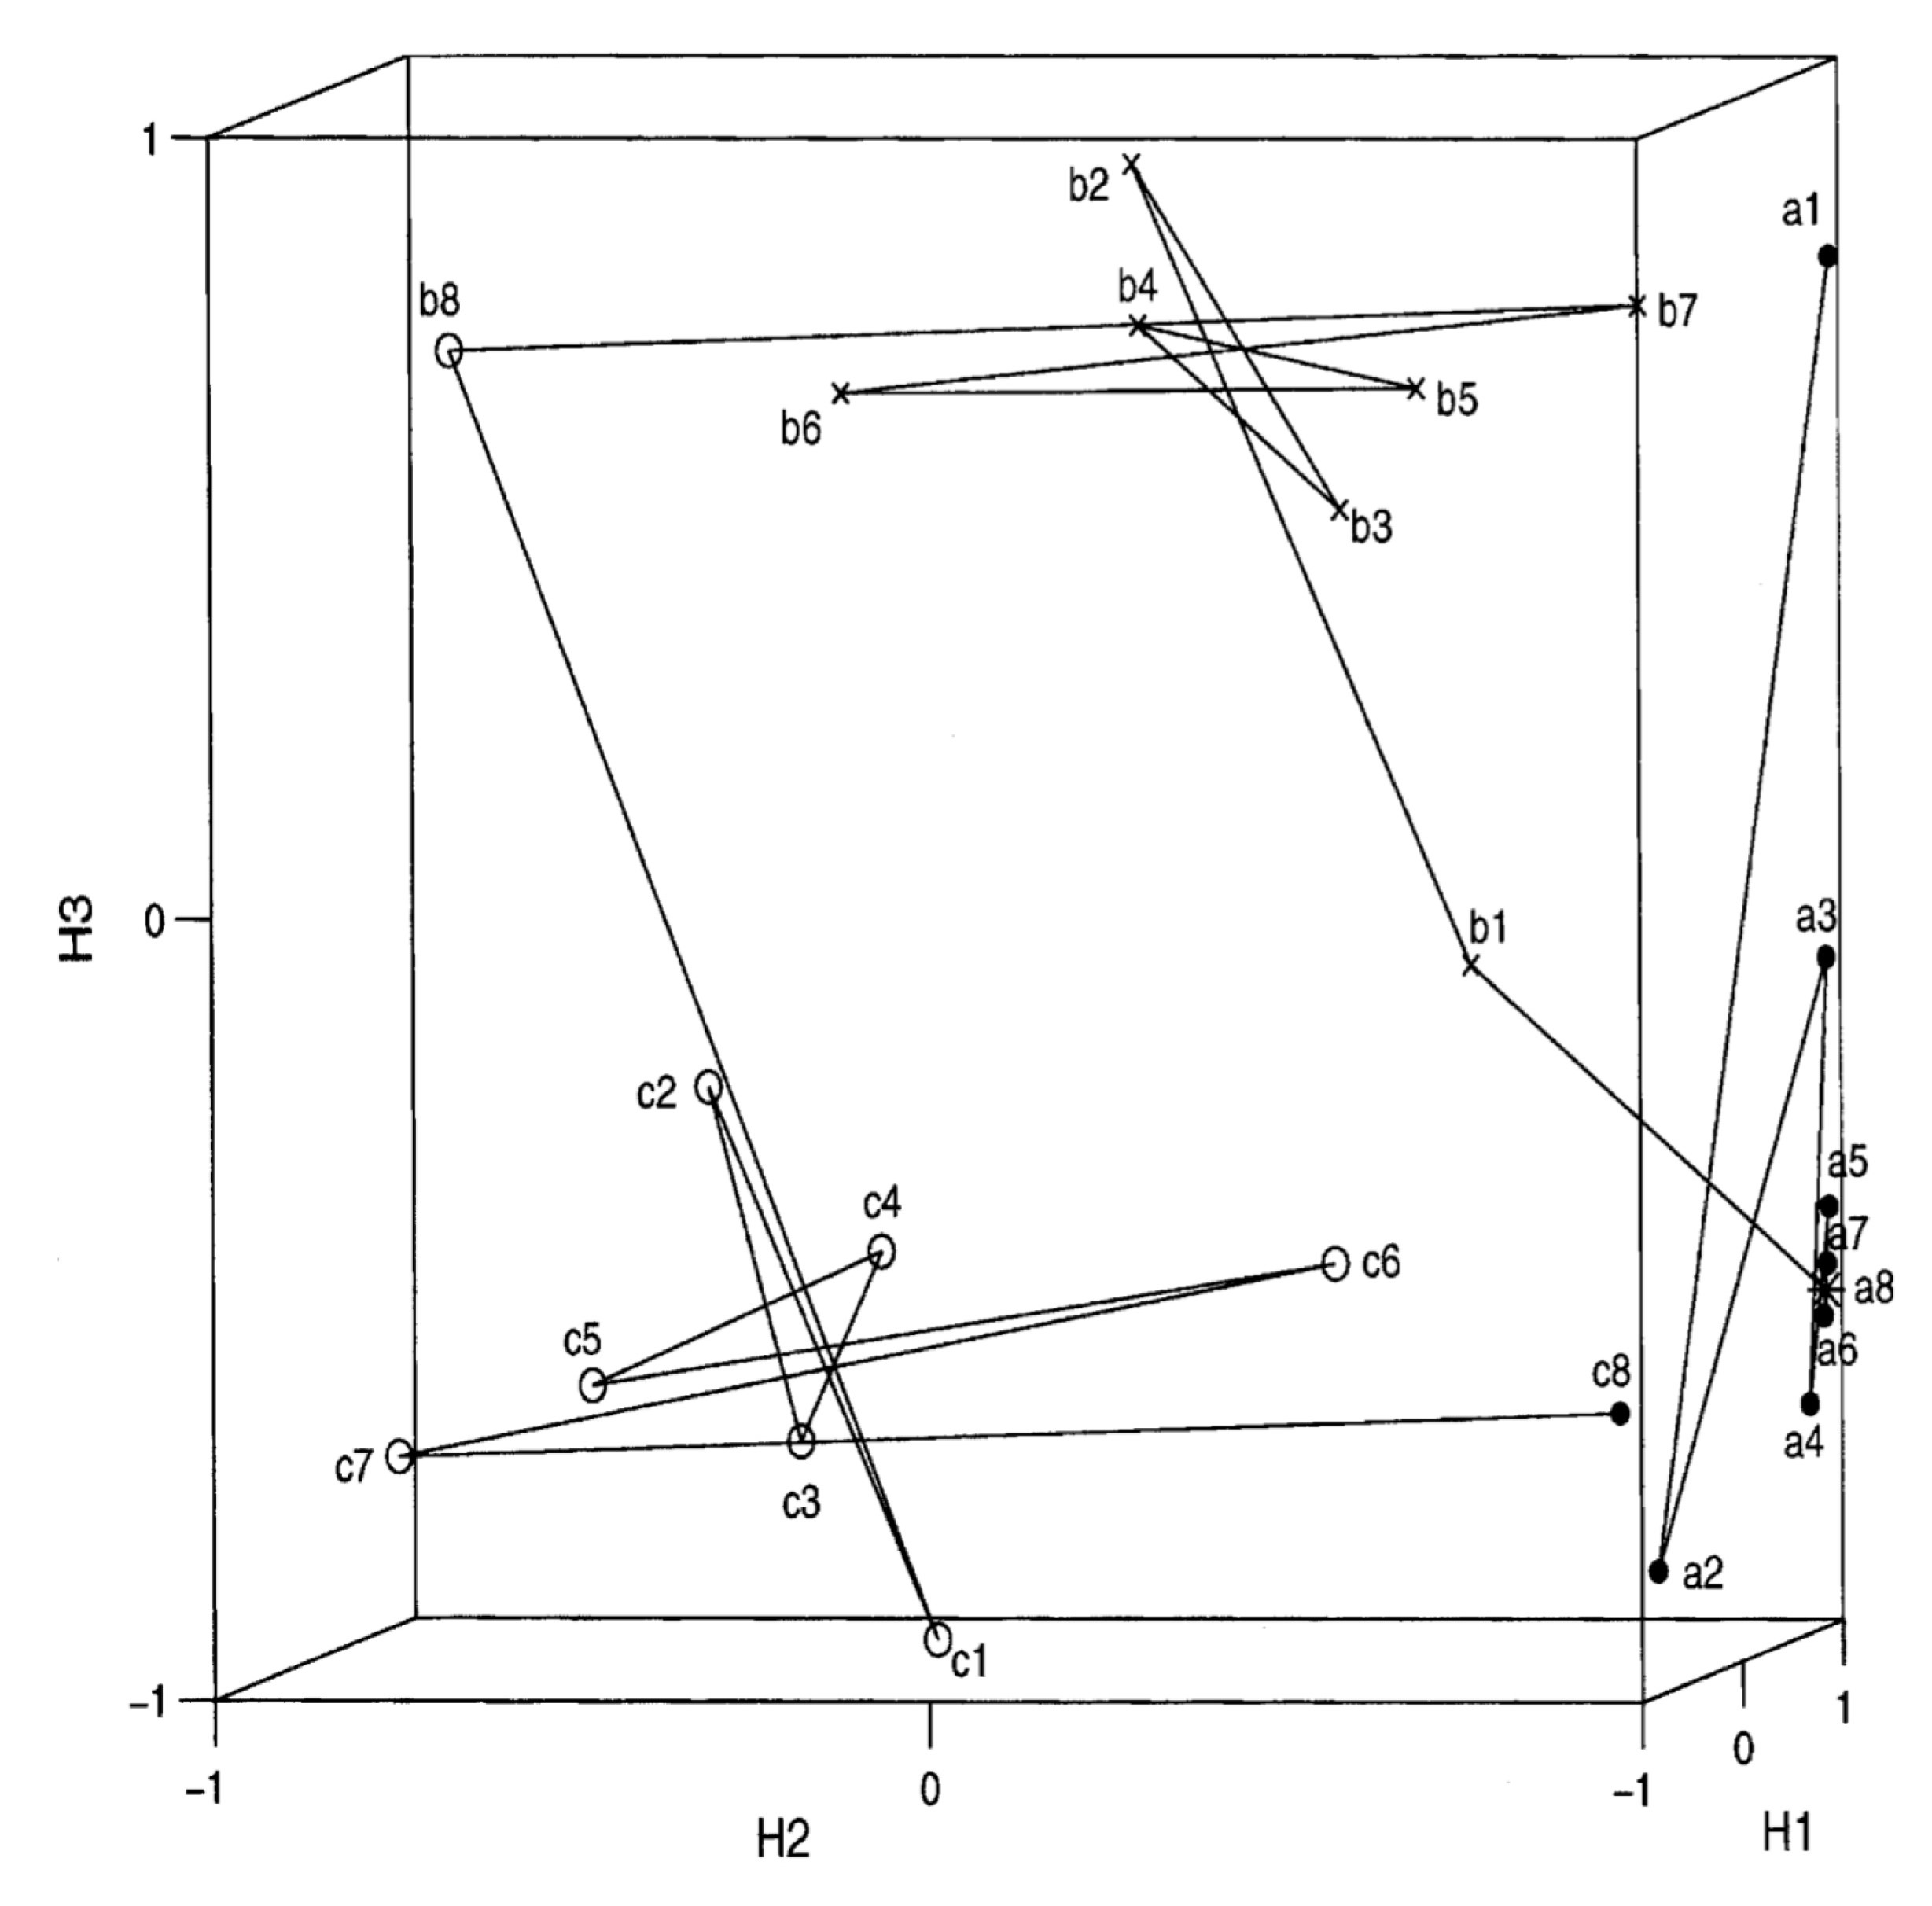
\includegraphics[width=12cm, height=8cm]{../out/images/hidden-unit-dynamics}
    \caption[hidden unit dynamics]{hidden unit dynamics}
    \label{fig: hidden unit dynamics}
\end{figure}

This analysis of network dynamics with simple languages is illuminating.
But, in the end, SRNs are limited in the range of dependencies they are able to
learn, for reasons analogous to the vanishing gradient problem which we
discussed in Week 2 in the context of feedforward networks.
In the next section we will introduce Long Short Term Memory, which is able to
learn longer range dependencies and $-$ in combination with word vectors,
attention and other enhancements $-$ can perform serious real world tasks such
as multilingual translation.

insert video

\section{Statistics of Language}\label{sec:statistics-of-language}
\subsection{Definitions, synonyms and antonyms}\label{subsec:definitions-synonyms-and-antonyms}

How do we capture the true meaning of a word, or its relationship to other
words?

Words are sometimes arranged into a taxonomy $-$ for example, a bird is a
mammal is an animal, etc.

We can also look at dictionary definitions, or lists of synonyms and antonyms.

Here is a list of synonyms for the word \('\)elegant\('\):

    stylish, graceful, tasteful, discerning, refined, sophisticated, dignified, cultivated, distinguished, classic, smart, fashionable, modish, decorous, beautiful, artistic, aesthetic, lovely; charming, polished, suave, urbane, cultured, dashing, debonair; luxurious, sumptuous, opulent, grand, plush, high-class, exquisite

Human effort is required to compile taxonomies, dictionary definitions and
lists of synonyms and antonyms.

Some important relationships may be missing, nuances may be lost.
Words like \('\)king\('\) and \('\)queen\('\) are not quite synonyms nor
antonyms because they are similar in some attributes but opposite in others.

Is it possible to extract statistical properties and relationships between
words automatically, without human involvement?

We will discuss a number of techniques for statistical language processing,
using this children's rhyme as an example.

There was a Crooked Man who walked a crooked mile and found a crooked sixpence
upon a crooked stile.
He bought a crooked cat, who caught a crooked mouse, and they all lived
together in a little crooked house.

\begin{figure}[H]
    \centering
    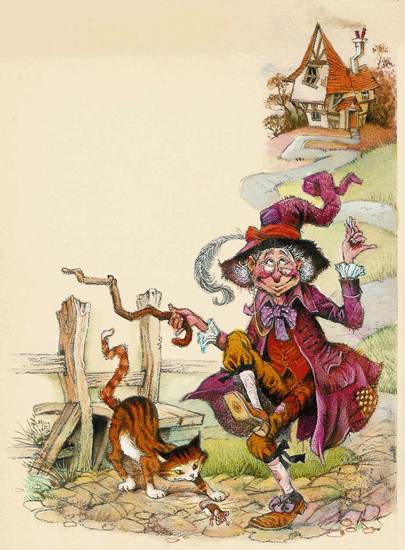
\includegraphics{../out/images/john_patience}
    \caption[john patience]{john patience}
    \label{fig:john patience}
\end{figure}

\section{Singular Value Composition}\label{sec:singular-value-composition}
\subsection{Counting word frequencies}\label{subsec:counting-word-frequencies}
Perhaps the simplest thing we can do to analyse a text is just to count the
frequency with which each word occurs.

\begin{figure}[H]
    \centering
    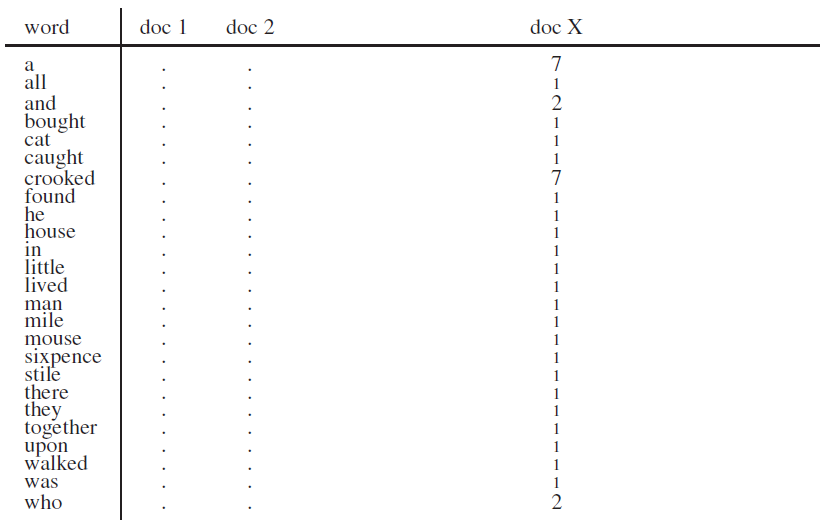
\includegraphics{../out/images/word-count}
    \caption[word count]{word count}
    \label{fig:word count}
\end{figure}

This can be useful for document classification.
Each column of the matrix becomes a vector representing the corresponding
document.
Some words like \('\)a\('\), \('\)and\('\) occur frequently in all (or most)
documents;
other words occur frequently only in certain types of documents, so are more
distinctive.
For example, words like \('\)cat\('\), \('\)mouse\('\), \('\)house\('\) tend
to occur in children’s books or rhymes, while other groups of words might be
characteristic of legal documents, political news, sporting results, etc.

Words occurring many times in one document may skew the vector.
Sometimes it is better if the matrix entries are just \('1'\) or \('0'\)
indicating whether the word occurs at all.

\subsection{counting consecutive words}\label{subsec:counting-consecutive-words}
Another thing we can do is to count the frequency of two words occurring
consecutively.

\begin{figure}[H]
    \centering
    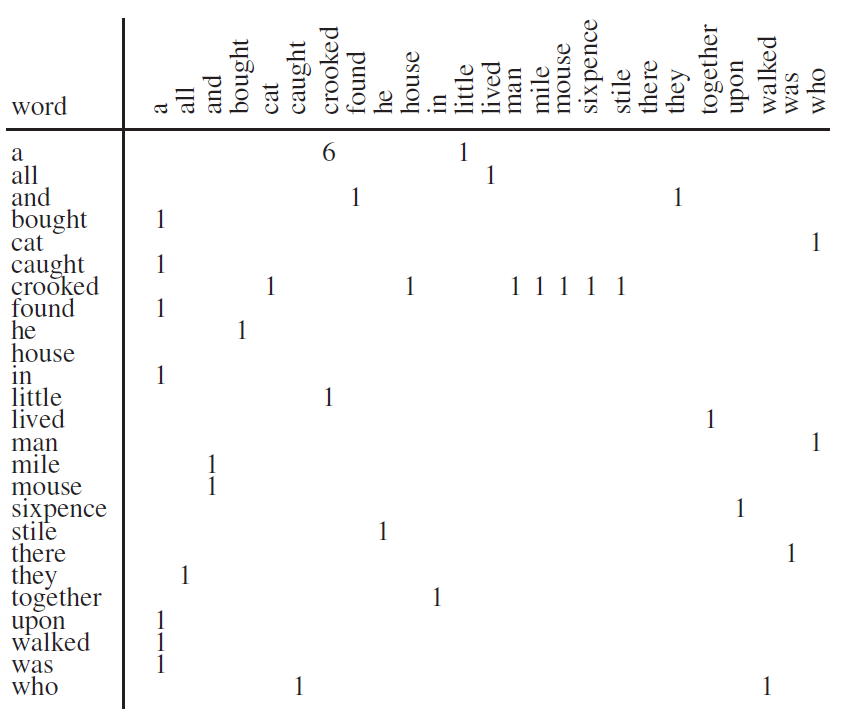
\includegraphics{../out/images/counting-consecutive-words}
    \caption[counting consecutive words]{counting consecutive words}
    \label{fig:counting consecutive words}
\end{figure}

\subsection{Predictive $n$-Gram Word Model}\label{subsec:predictive-$n$-gram-word-model}
If we normalise so that the sum of the entries in each row is equal to $1$, we
can use this matrix to estimate the probability $prob(w_j | w_i)$ of word $w_j$
occurring after $w_i$

\begin{figure}[H]
    \centering
    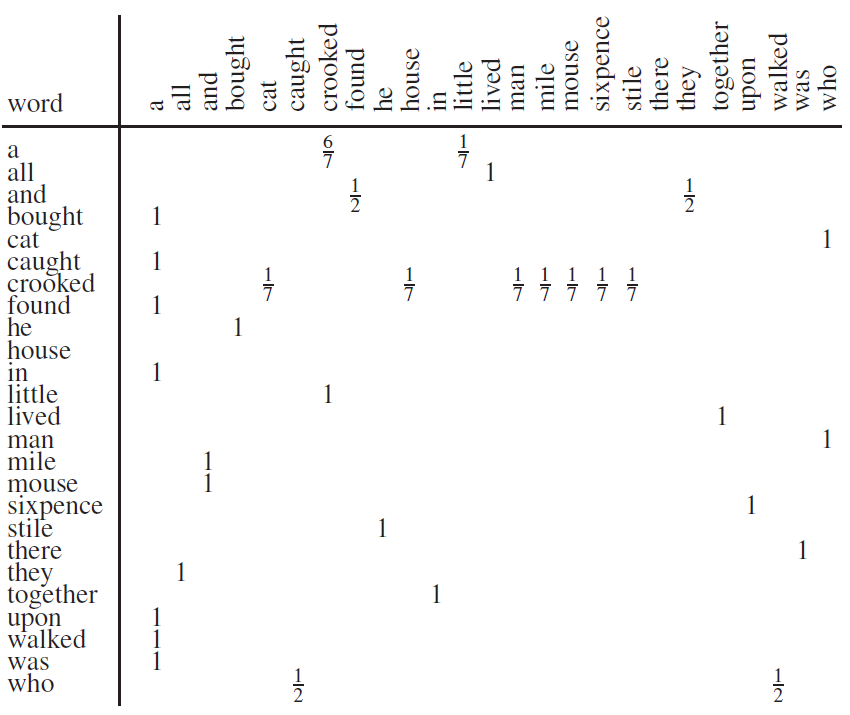
\includegraphics{../out/images/predictive-n-gram-word-model}
    \caption[predictive n-gram word model]{predictive n-gram word model}
    \label{fig:predictive n-gram word model}
\end{figure}

In practice, we need to aggregate over a large corpus, so that unusual words
like \("\)crooked\("\) will not dominate.

The above model captures some common combinations like “there was”, “man who”,
“and found”, “he bought”, “who caught”, “and they”, “they all”, “lived
together”, etc.

This unigram model can be generalised to a bi-gram, tri-gram, .
. . , $n$-gram model by considering the nnn preceding words.
If the vocabulary is large, we need some tricks to avoid exponential use of memory.

\subsection{Unigram Text Generator}\label{subsec:unigram-text-generator}
Here is an example of text generated from a unigram model based on the
frequencies of word pairs in Shakespeare's Hamlet.

“Rashly – Good night is very liberal – it is easily said there is – gyved to a
sore distraction in wrath and with my king may choose but none of shapes and
editing by this, and shows a sea And what this is miching malhecho;
And gins to me a pass, Transports his wit, Hamlet, my arms against the mind
impatient, by the conditions that would fain know;
which, the wicked deed to get from a deed to your tutor.”

We see that the local structure looks plausible, but the global structure seems
like gibberish.

\subsection{Co-occurrence Matrix}\label{subsec:co-occurrence-matrix}
Sometimes, we don’t necessarily predict the next word, but simply a “nearby
word” (e.g.\ a word occurring within an $n$-word window centered on that word).

For this case, we can build a matrix in which each row represents a word, and each column a nearby word.
Co-occurrence Matrix (2-word window)

\subsection{Co-occurrence Matrix (10-word window)}\label{subsec:co-occurrence-matrix-(10-word-window)}
\begin{figure}[H]
    \centering
    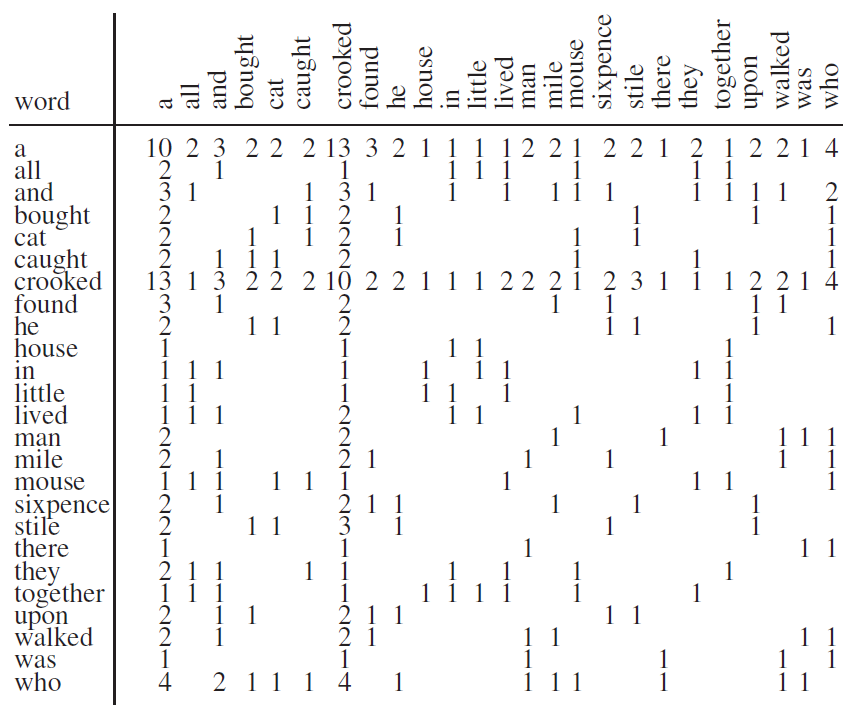
\includegraphics{../out/images/co-occurence-matrix}
    \caption[co-occurence matrix]{co-occurence matrix}
    \label{fig:co-occurence matrix}
\end{figure}
By aggregating over many documents, pairs (or groups) of words emerge which
tend to occur near each other (but not necessarily consecutively).
For example:
- \('\)cat\('\), \('\)caught\('\), \('\)mouse\('\)
- \('\)walked\('\), \('\)mile\('\)
- \('\)little\('\), \('\)house\('\)

This analysis raises a number of questions:
- Common words tend to dominate the matrix.
Could we sample common words less often, in order to reveal the relationships
of less common words?
- Each row of this matrix could be considered as a vector representation for
the corresponding word, but the number of dimensions is equal to the size of
the vocabulary, which could be very large (∼ 10510^5105).
- Is there a way to reduce the dimensionality while still preserving the
relationships between words?

\subsection{Optional Video}\label{subsec:optional-video}

\section{Singular Value Decomposition}\label{sec:singular-value-decomposition}
\subsection{Word Vectors}\label{subsec:word-vectors}
\textif{“Words that are used and occur in the same contexts tend to purport similar meanings.”} Z. Harris (1954)
\textif{“You shall know a word by the company it keeps.”} J.R.\ Firth (1957)
We would like to assign a vector to each word or document, in such a way that
words with nearby representations are likely to occur in similar contexts (or,
similar documents have close vectors).

Each column in the co-occurrence matrix could be considered as a vector
representation of a word or document.
However, the number of dimensions in this vector would be very large (equal to
the size of the vocabulary, which is typically about 60,000).

Singular Value Decomposition (SVD) is a way of projecting these vectors from
60,000 dimensions to about 200 dimensions, in such a way that the relationship
between words (or documents) is preserved.
SVD itself is too computationally expensive, so methods like Word2Vec and Glove
are introduced which provide a good approximation to SVD with reasonable
computing resources.

\subsection{Singular Value Decomposition}\label{subsec:singular-value-decomposition2}
Let $X$ be a (co-)occurrence matrix where each row represents a word, and each
column represents either a word (in which case  or a document (in which case
$L$, might not be equal).

This matrix  can be decomposed as where $X = USV^T$ where $U_{(L \times L)}, V_{(M \times M)}$ are unitary (all columns have unit length) and $S_{L \times M}$ is diagonal, with diagonal entries $s_1 \geq s_2 \geq \dots \geq s_M \geq 0$

\begin{figure}[H]
    \centering
    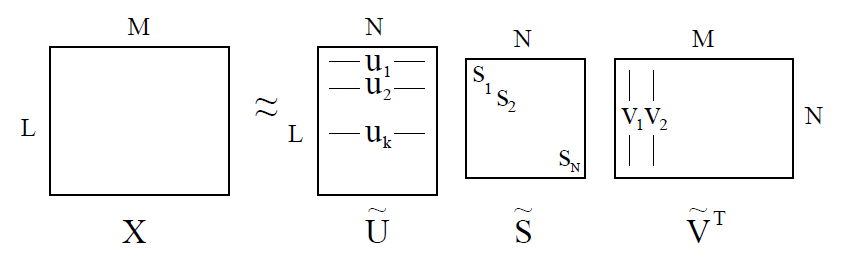
\includegraphics{../out/images/singular-value-decomposition}
    \caption[singular value decomposition]{singular value decomposition}
    \label{fig:singular value decomposition}
\end{figure}

We can obtain an approximation for $X$ of rand $N < M$ by truncating $U$ to
$\tilde{U}_{L \times N}$, $S$ to $\tilde{S}_{(N \times N)})$ and $V$ to
$\tilde{V}_{(M \times N)}$.
The $k^{th}$ row of $U$ then provides an N-dimensional vector representing the
$k^{th}$ word in the vocabulary.
The $k^{th}$ column of $\tilde{V}^T$ also provides an N-dimensional vector,
which can be seen either as a representation for documents, or as an
alternative representation for words, depending on the origin of the
(co-)occurrence matrix.

\subsection{Word2vec and GloVe}\label{subsec:word2vec-and-glove}
Typically, is the number of words in the vocabulary (about 60,000) and $M$ is
either equal to $L$ or, in the case of document classification, the number of
documents in the collection.
SVD is computationally expensive, proportional to $L \times M^2$ if $L \geq M$

word2vec (Mikolov, 2013) and GloVe (Pennington, 2014) are two common methods for computing an approximation to SVD incrementally, with less computation.
\textbf{word2vec} is a predictive model which aims to maximise the probability of a word, based on the surrounding words.
\textbf{GloVe} is a count-based model which tries to directly reconstruct a close approximation to the co-occurrence matrix $X$.

\subsection{Singular Value compared to Eigenvalue Decomposition}\label{subsec:singular-value-compared-to-eigenvalue-decomposition}
Those familiar with Eigenvalue Decomposition will see that it is similar in some ways to Singular Value Decomposition.
But, we must note a number of important differences, as illustrated in these examples:

Eigenvalue Decomposition
\[\]

Single Value Decomposition
\[\]

\subsection{Singular Value Decomposition}\label{subsec:singular-value-decomposition}:

In general, eigenvalues can be negative or even complex, but singular values are always real and non-negative.
Even if $X$ is a square matrix, singular value decomposition treats the source and target as two entirely different spaces.
The only case where the two decompositions are the same is when $X$ is symmetric and positive semi-definite.
The word co-occurrence matrix is symmetric but not positive semi-definite.
For example, if the text consisted entirely of two alternating letters ..ABABABABABABAB.. then A would be the context for B, and vice-versa.

\subsection{Optional Video}\label{subsec:optional-video2}

\section{Word2Vec}\label{sec:word2vec}
\begin{figure}[H]
    \centering
    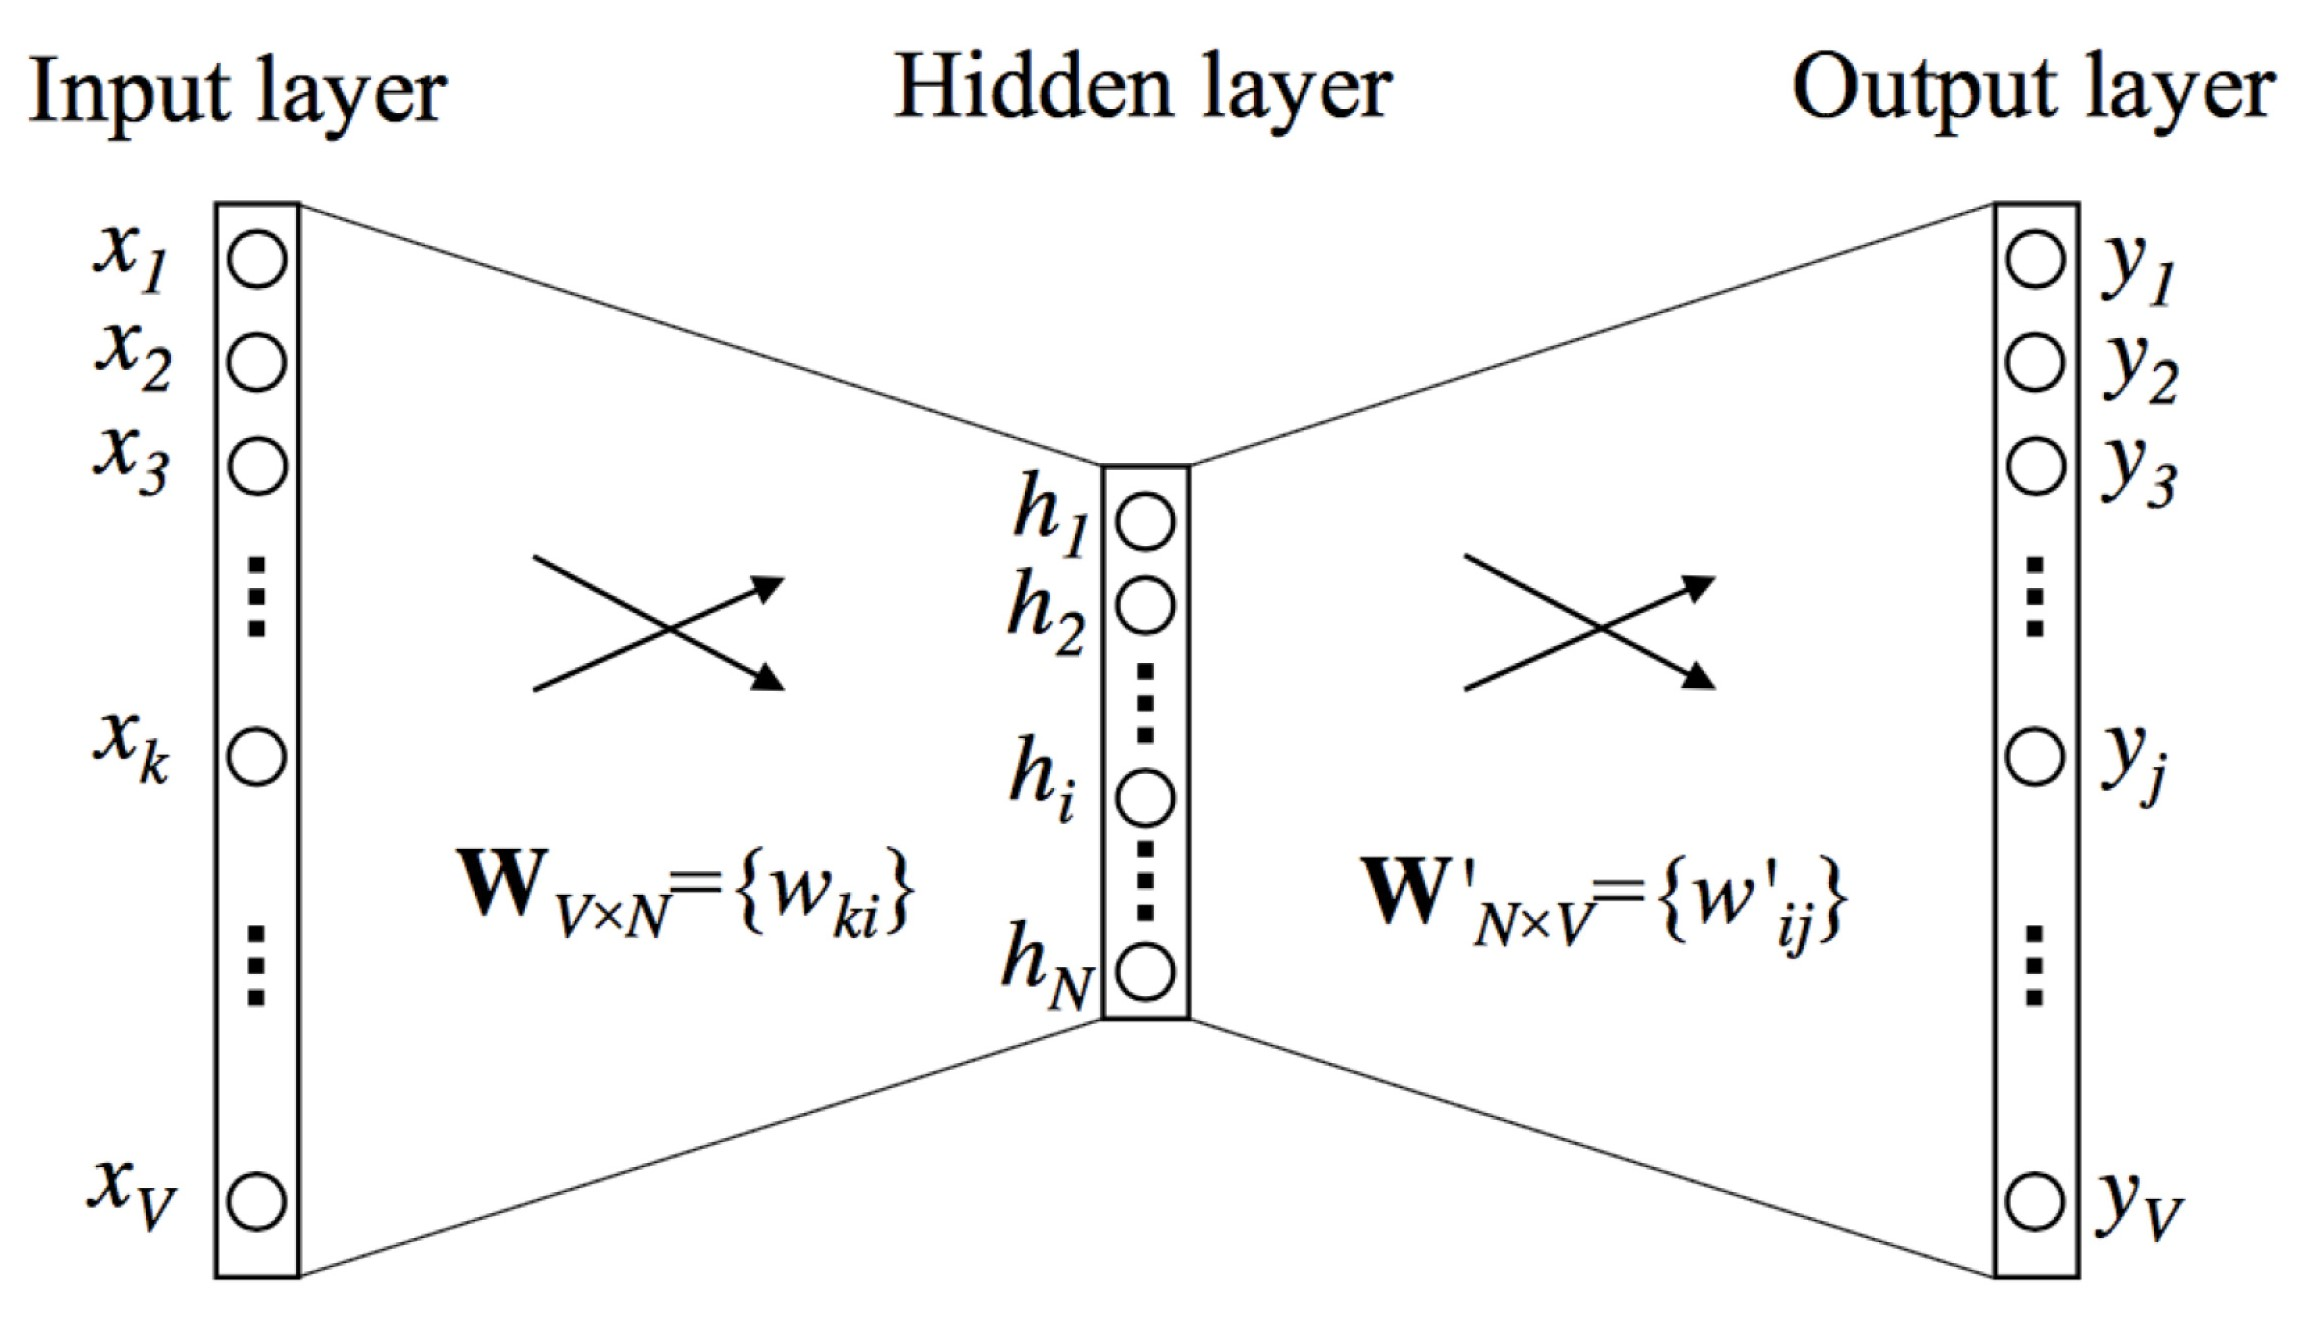
\includegraphics{../out/images/word2vec}
    \caption[word2vec]{word2vec}
    \label{fig:word2vec}
\end{figure}

The $k^{th}$ row $$ of $W$ is a representation of word $k$.

The $$ is an (alternative) representation of word $j$.

If the (1-hot) input is $k$, the linear sum at each output will be

Note that word2vec is a linear model in the sense that there is no activation
function at the hidden nodes.

\subsection{Cost function}\label{subsec:cost-function}
Softmax can be used to turn these linear sums  into a probability distribution
estimating the probability of word $j$ occurring in the context of word $k$

We can treat the text as a sequence of numbers $a$ means that the $b$ word in
the text is the $c$ word in the vocabulary.

We then seek to maximise the log probability

where ccc is the size of training context (which may depend on .

\subsection{word2vec differentials}\label{subsec:word2vec-differentials}
If we assume the probabilities are computed by full softmax, and the correct
output is $j\astj^\astj\ast$, then the cost function is

the output differentials are

where

\subsection{word2vec weight updates}\label{subsec:word2vec-weight-updates}

\subsection{hidden-to-output differentials}\label{subsec:hidden-to-output-differentials}

\subsection{hidden unit differentials}\label{subsec:hidden-unit-differentials}

\subsection{input-to-hidden differentials}\label{subsec:input-to-hidden-differentials}

\subsection{Continuous Bag of Words and Skip-Gram}\label{subsec:continuous-bag-of-words-and-skip-gram}
word2vec can be implemented either as Continuous Bag of Words (CBOW) or Skip-Gram, as illustrated in these figures from [Rong, 2014].

\begin{figure}[H]
    \centering
    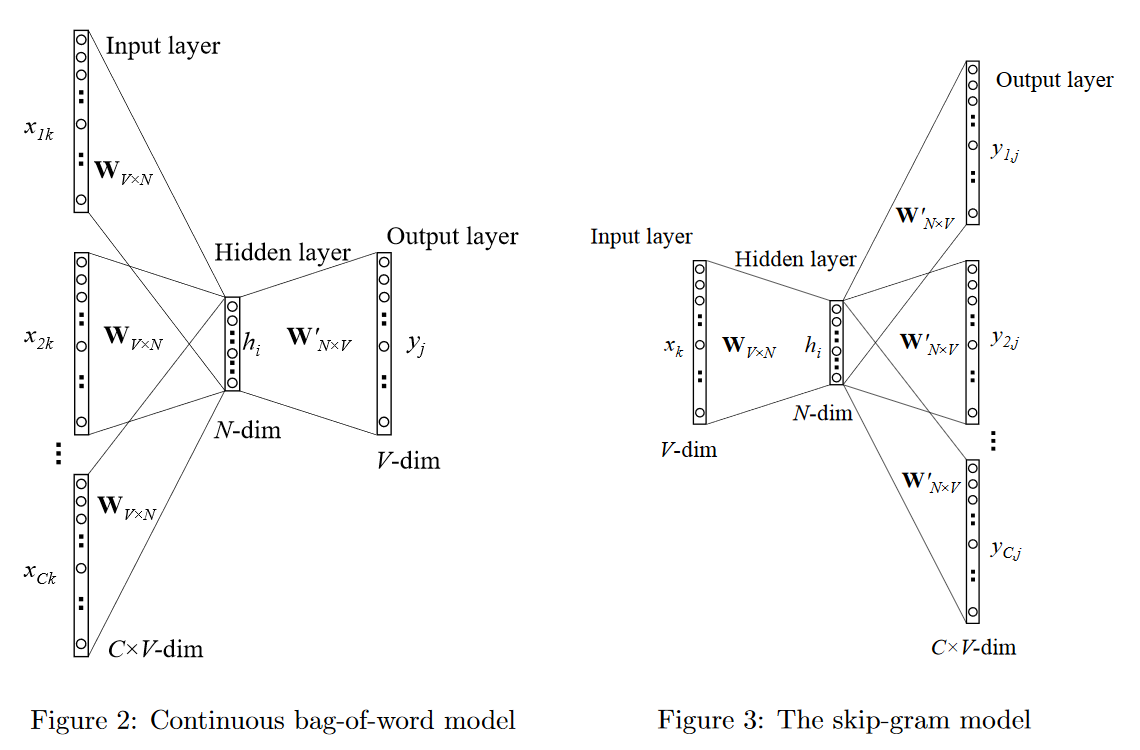
\includegraphics{../out/images/continuous-bag-of-words}
    \caption[continuous bag of words]{continuous bag of words}
    \label{fig:continuous bag of words}
\end{figure}

For CBOW, several context words are each used independently to predict the
centre word, and the hidden activation becomes a sum (or average) over all the
context words.

Note the difference between this and NetTalk $-$ in word2vec (CBOW) all context
words share the same input-to-hidden weights.

The Skip-Gram version tries to predict the context words, given the centre
word.
This is similar to CBOW, except that in this case a single input word is used
to predict multiple context words, and all context words share the same
hidden-to-output weights.

\subsection{Efficiency issues}\label{subsec:efficiency-issues}
Depending on the computational resources available, it may be prohibitively
expensive to use the full softmax, which involves computing output values for
all 60,000 words in the vocabulary.
Hierarchical Softmax and negative sampling are two alternatives which are
computationally more efficient.

\subsection{Hierarchical Softmax}\label{subsec:hierarchical-softmax}
For Hierarchical Softmax, the words are arranged in a Huffmann coded tree
according to their frequency.
One network output (with sigmoid activation) is assigned to each node in the
tree, and the output corresponding to each node in the path from the root to
the actual word is trained to produce either 0 or 1 depending on whether the
left or right branch should be taken.
In this way, the total number of outputs is the same, but if the size of the
vocabulary is $L$ then only $\log_2(L)$ outputs need to be evaluated, on
average, for each word in the training text.

\subsection{Negative sampling}\label{subsec:negative-sampling}
The idea of negative sampling is that we train the network to increase its
estimation of the target word j∗j^*j∗ and reduce its estimate not of all the
words in the entire vocabulary but instead just a subset of them, drawn from an
appropriate distribution.

\[E = -\log \sigma(v'_{j*}^T) - \sum_{j \in W_{neg}} \log \sigma (-v'_{j}^{T}h)\]

This is a simplified version of Noise Contrastive Estimation (NCE).
It is not guaranteed to produce a well-defined probability distribution, but in
practice it does produce high-quality word embeddings.

The number of samples is 5--20 for small datasets, 2--5 for large datasets.

Empirically, a good choice of the distribution from which to draw the negative
samples is $P(w) = U(w)^{3/4} / Z$ where $U(w)$ is the unigram distribution
determined by the previous word, and $Z$ is a normalizing constant.

\subsection{Subsampling of frequent words}\label{subsec:subsampling-of-frequent-words}
In order to diminish the influence of more frequent words, each word in the
corpus is discarded with probability

\[P(w_i) = 1 - \sqrt{\dfrac{t}{f(w_i)}}\]

where $f(w_i)$ is the frequency of word $t ~ 10^{-5}$ is an empirically
determined threshold.

\subsection{Optional Video}\label{subsec:optional-video3}

\section{Word Relationships}\label{sec:word-relationships}
\subsection{Sentence Completion Task}\label{subsec:sentence-completion-task}

One way to test the quality of the word embeddings is by using them to answer
sentence completion tasks from standardised tests such as the Scholastic
Aptitude Test (SAT).

\textbf{Q1}
Seeing the pictures of our old home made me feel \_______ and nostalgic.

\begin{itemize}
  \item A. fastidious
  \item B. indignant
  \item C. wistful
  \item D. conciliatory
\end{itemize}

This kind of question can be answered by feeding the surrounding words into the CBOW version of the network and seeing which of  is assigned the highest probability by the network.

\textbf{Q2}
Because the House had the votes to override a presidential veto, the President has no choice but to _\___________ .

\begin{itemize}
  \item A. object
  \item B. abdicate
  \item C. abstain
  \item D. compromise
\end{itemize}

The network might have some difficulty answering questions like Q2, because of
the need for logical reasoning or culturally specific knowledge.

\section{Word Relationships}\label{sec:word-relationships2}
Another way to probe the word vectors is to look for linguistic regularities.
For example, if we add the vectors for $\text{King}$ and $\text{Woman}$ and
subtract the vector for $\text{Man}$, we get something very close to the vector
for $\text{Queen}$, i.e.

\[\text{King} + \text{Woman} - \text{Man} \simeq \text{Queen}\]

This can be used to answer questions of the form: $A$ is to $B$ as $B$ is to
What?
For example:

\textbf{Q3}
evening is to morning as dinner is to _______ .
\begin{itemize}
  \item A. breakfast
  \item B. soup
  \item C. coffee
  \item D. time
\end{itemize}

\text{Q4}
bow is to arrow as ______ is to bullet.

\begin{itemize}
  \item A. defend
  \item B. lead
  \item C. shoot
  \item D. gun
\end{itemize}

In each case, we look for the word $X$ in the dictionary whose vector is closest to $(v_C + v_B - v_A)$, with closeness determined by cosine similarity.

\[X = \arg \max \dfrac{(v_C + v_B -v_A)^T v_X}{||v_C + v_B -v_A||}\]

Here are some examples of word relationships from (Mikolov, 2013).

\begin{figure}[h]
    \centering
    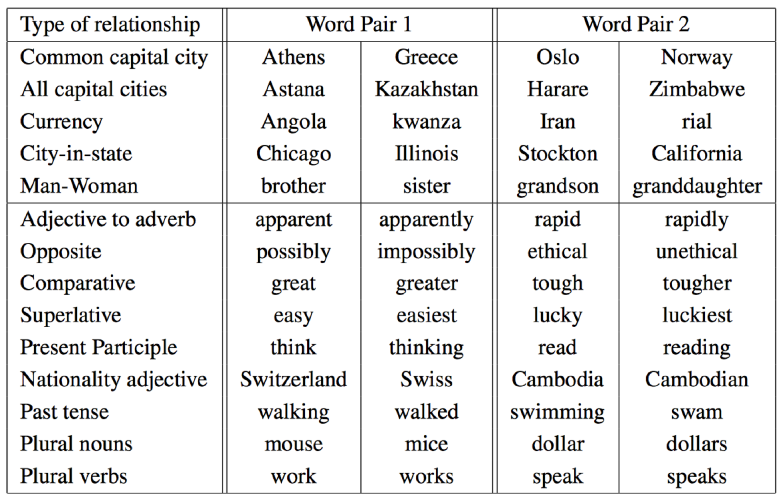
\includegraphics[width=12,height=12]{../out/images/word-relationships}
    \caption[word relationships]{word relationships}
    \label{fig:word relationships}
\end{figure}

\begin{figure}[h]
    \centering
    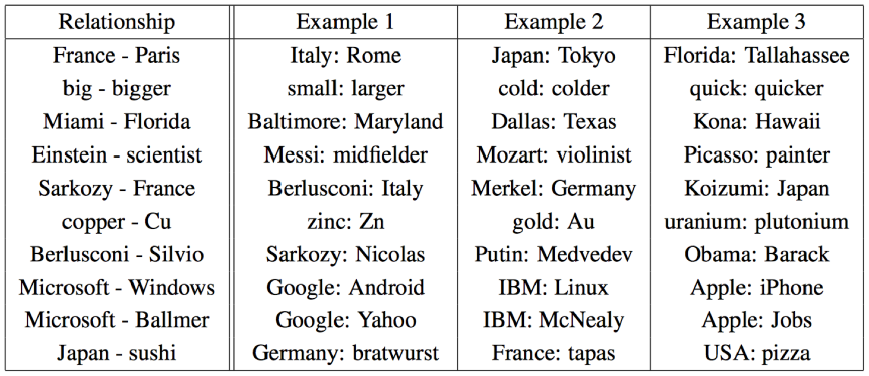
\includegraphics[width=12,height=12]{../out/images/word-relationships-2}
    \caption[word relationships 2]{word relationships 2}
    \label{fig:word relationships 2}
\end{figure}

The network generally performs very well, but occasionally makes an
understandable mistake.
For example, did you notice what the network thinks is the first and last name
of the President of Russia?

\subsection{Optional Video}\label{subsec:optional-video4}

\section{Exercises}\label{sec:exercises}
Consider the sentence:
\textif{"two flowers grew tall on two tall towers"}

\textbf{Question 1}
Write the co-occurrence matrix $X$ for this sentence, using a 4-word context
window (i.e.\ two context words on either side of the central word).

\textbf{Answer}
\begin{center}
\begin{tabular}{ |c|c|c| }
 \hline
  & flowers & grew & on & tall & towers & two \\
 flowers & 0 & 1 & 0 & 1 & 0 & 1 \\
 grew & 1 & 0 & 1 & 1 & 0 & 1 \\
 on & 0 & 1 & 0 & 2 & 0 & 1 \\
 tall & 1 & 1 & 2 & 0 & 1 & 2 \\
 towers & 0 & 0 & 0 & 1 & 0 & 1 \\
 two & 1 & 1 & 1 & 2 & 1 & 0 \\
 \hline
\end{tabular}
\end{center}

\textbf{Question 2}
Use `torch.svd()` to compute the singular value decomposition of this matrix
$X = UST^T$.

\textbf{Answer}
see .py file
\textbf{Note: replacing U and V with -U and -V would also preserve $X=USV^T$}

\textbf{Question 3}
Extract a word representation from the first two columns of $U$ and use
matplotlib to plot the words on a 2-dimensional graph.

\textbf{Answer}
see .py file
\textbf{Note: the image may be rotated dependign on the sign of $U$}
\part{4d language processing}\label{part:4d-language-processing}

\section{Discussion: Translation, Transformers and ChatBots}\label{sec:discussion:-translation-transformers-and-chatbots}

\begin{figure}[h]
    \centering
    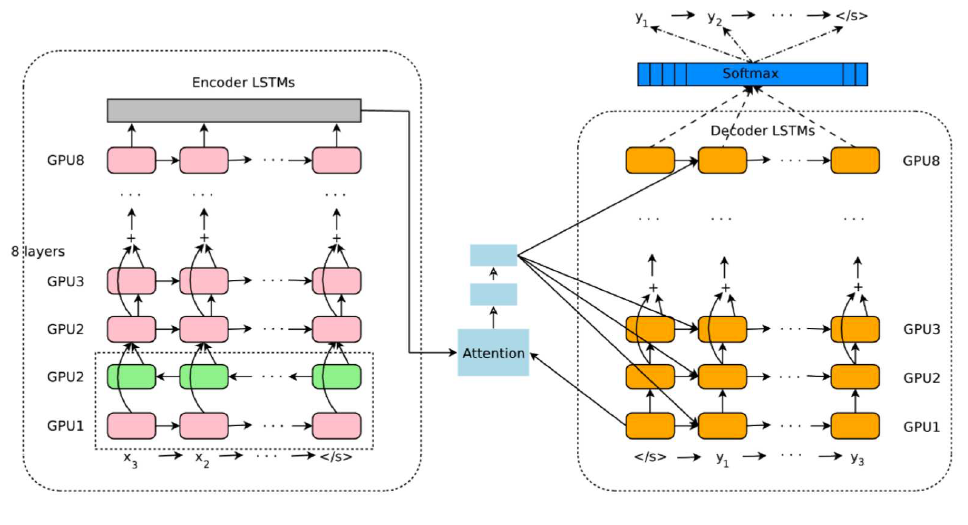
\includegraphics[]{../out/images/attention-mechanism}
    \caption[attention mechanism]{attention mechanism}
    \label{fig:attention mechanism}
\end{figure}

These articles explain how an attention mechanism can be used for
sequence-to-sequence prediction, and how stacked LSTMs, combined with attention
and word vectors, can be used for multilingual neural machine translation:

\subsection{Transformers and GPT-3}\label{subsec:transformers-and-gpt-3}
Transformers like GPT-3 have recently achieved very impressive results on text
prediction, as described in these resources:

\subsection{Recommended discussion}\label{subsec:recommended-discussion}
Recommended discussion

In the Ed discussion board, write a brief post in the category Lessons - Week 7
outlining your thoughts on the following three points.
Then reply to at least one other person's post and read through others to
consider multiple viewpoints.
\begin{itemize}
  \item Do you believe GPT-3 is really producing \("\)original\("\) material, or is it just \("\)mashing\("\) existing texts together in a deep way?
  \item What will be the implications of systems like GPT-3 on issues such as journalism, commentary, copyright, authorship, plagiarism, education?
  \item Until recently, major companies were still using traditional scripting for their chat-bots, rather than deep neural networks. One motivation for this might be to avoid problems such as those manifested by Microsoft's Tay system in 2016.
\end{itemize}

Do you think chatbots in the future might be based on transformers and other
deep learning architectures?
If so, how could they avoid becoming inappropriately rude, offensive,
misleading, deceptive or impertinent?

    insert video

\section{Long Short Term Memory}\label{sec:long-short-term-memory}

Simple Recurrent Networks (SRNs) can learn medium-range dependencies but have
difficulty learning long range dependencies.
Long Short Term Memory (LSTM) is able to learn long range dependencies using a
combination of forget, input and output gates (Hochreiter and Schmidhuber, 1998).

\begin{figure}[h]
    \centering
    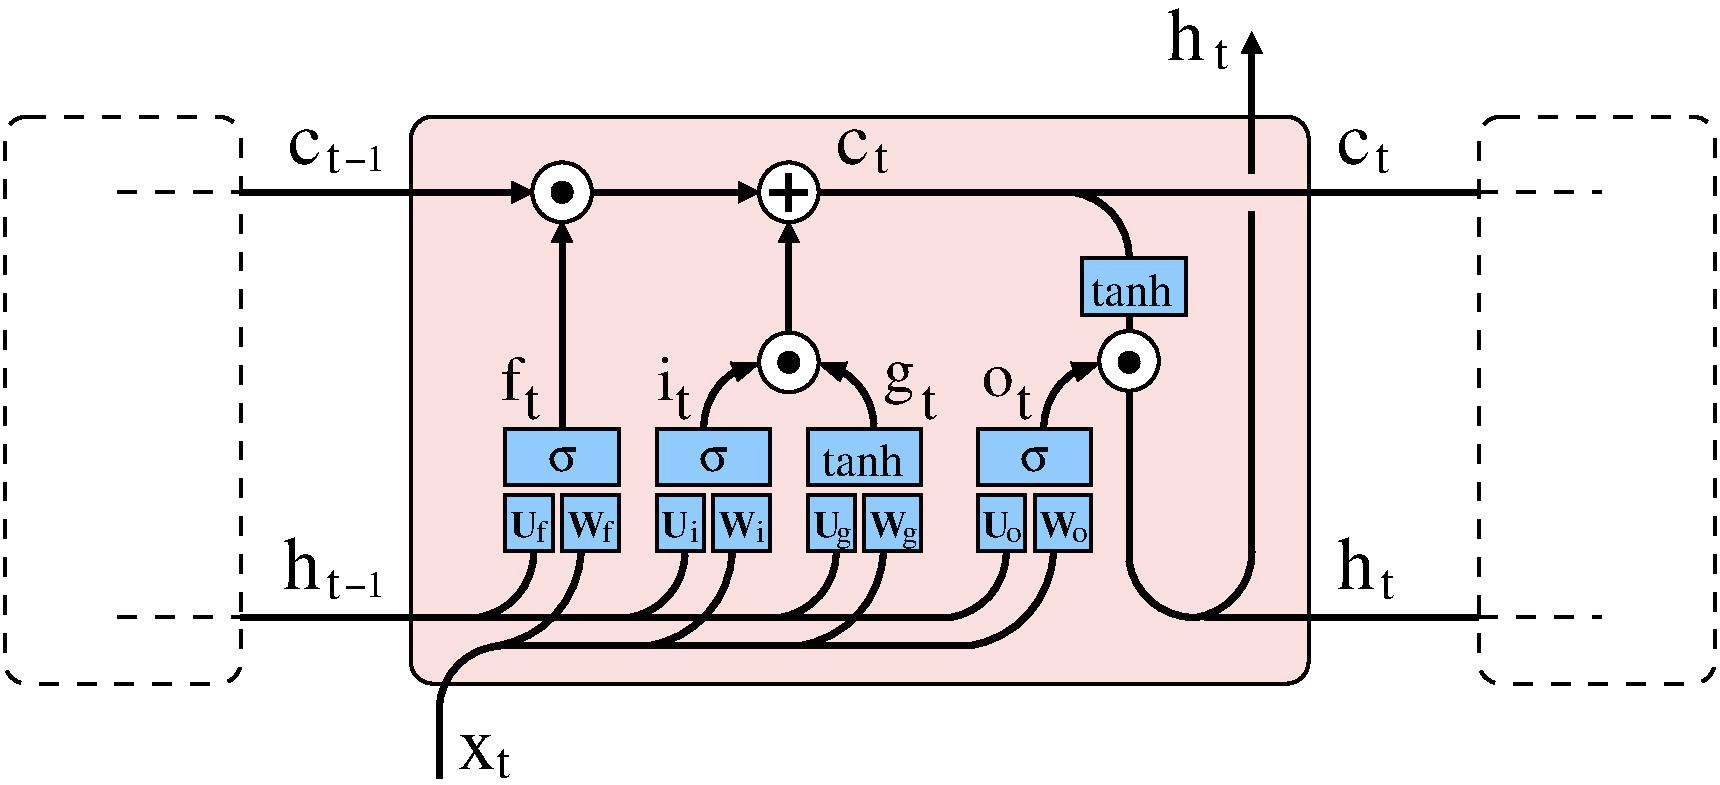
\includegraphics[width=12,height=8]{../out/images/lstm}
    \caption[LSTM]{LSTM}
    \label{fig: LSTM}
\end{figure}

The LSTM maintains a context layer which is distinct from the hidden layer but
contains the same number of units.
The full workings of the LSTM at each timestep are described by these
equations:

\textbf{Gates}

\begin{gather*}
    f_t = \sigma (U_f h_{t-1} + W_{f X_t} + b_f)\\
    i_t = \sigma(U_i h_{t-1} W_{i X_t} + b_i)\\
    o_i = \sigma(U_o h_{t-1} + W_{o X_t} + b_o)\\
\end{gather*}

\textbf{Candidate activation}

\[g_t = \tanh (U_g h_{t-1} + W_{g X_t})\]

\textbf{State}

\[c_t = f_t \odot c_{t-1} + i_t \odot g_t\]

\textbf{Outputs}:

\[h_t = o_t \odot \tanh c_t\]

First, the **forget** gate ($f$) is used to determine, for each context unit,
a ratio between 0 and 1 by which the value of this context unit will be
multiplied.
If the ratio is close to zero, the previous value of the corresponding context
unit will be largely forgotten;
if it is close to 1, the previous value will be largely preserved.

Next, \textbf{update} values ($g$) between $-1$ and $+1$ are computed using
$\tanh$, and the input gate ($i$) is used to determine ratios by which these
update values will be multiplied before being added to the current context
values.

Finally, the \textbf{output} gate ($o$) is computed and used to determine the
ratios by which $\tanh$ of the context unit values will be multiplied in order
to produce the next hidden unit values.

In this way, the context units are able to specialise, with some of them
changing their values frequently while others preserve their state for many
timesteps, until particular circumstances cause the gates to be opened and
allow the value of those units to change.

\subsection{Embedded Reber Grammar}\label{subsec:embedded-reber-grammar}

The ability of different sequence processing algorithms to learn long range
dependencies can be explored using the Reber Grammar and Embedded Reber Grammar.
\begin{figure}[h]
    \centering
    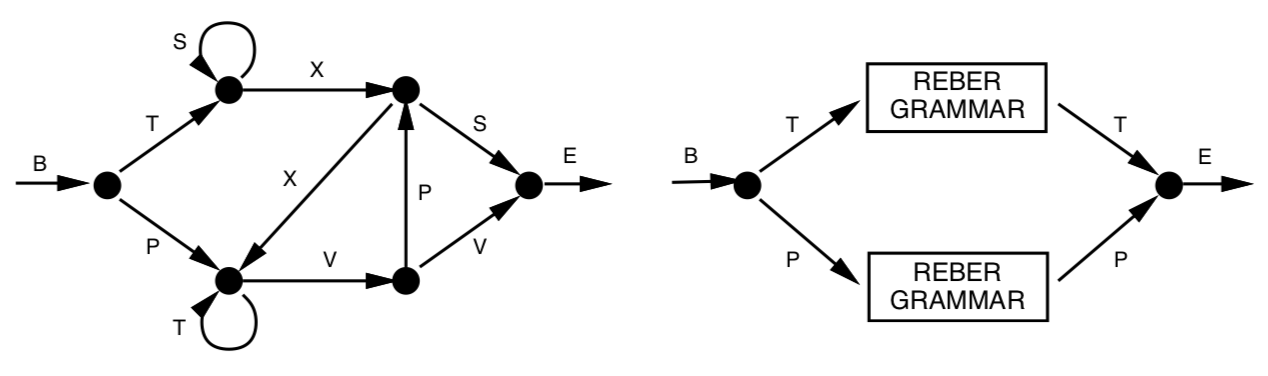
\includegraphics[width=12,height=4]{../out/images/reber-grammar}
    \caption[reber grammar]{reber grammar}
    \label{fig: reber grammar}
\end{figure}

The Reber Grammar (RG) is defined by the finite state machine shown on the left.
When there is a choice between two transitions, they are understood to be
chosen with equal probability.
The Embedded Reber Grammar (ERG) is shown on the right, where each box marked
\textbf{REBER GRAMMAR} contains an identical copy of the finite state machine
on the left.
The difficulty in learning the ERG is that the network must remember which
transition (T or P)  occurred after the initial B, and retain this information
while it is processing the transitions associated with the RG in one of the two
identical boxes, in order to correctly predict the T or P occurring before the
final E.

In the exercises for this week, you will be demonstrating that the SRN is able
to learn the RG but struggles to learn the ERG, whereas the LSTM can also learn
the ERG. We can imagine that one of the context units is somehow assigned the
task of retaining the knowledge of the initial T or P, and that this knowledge
is preserved by appropriately high and low values for the forget gate and the
input and output gate, respectively.

\subsection{Gated Recurrent Unit}\label{subsec:gated-recurrent-unit}

\begin{figure}[h]
    \centering
    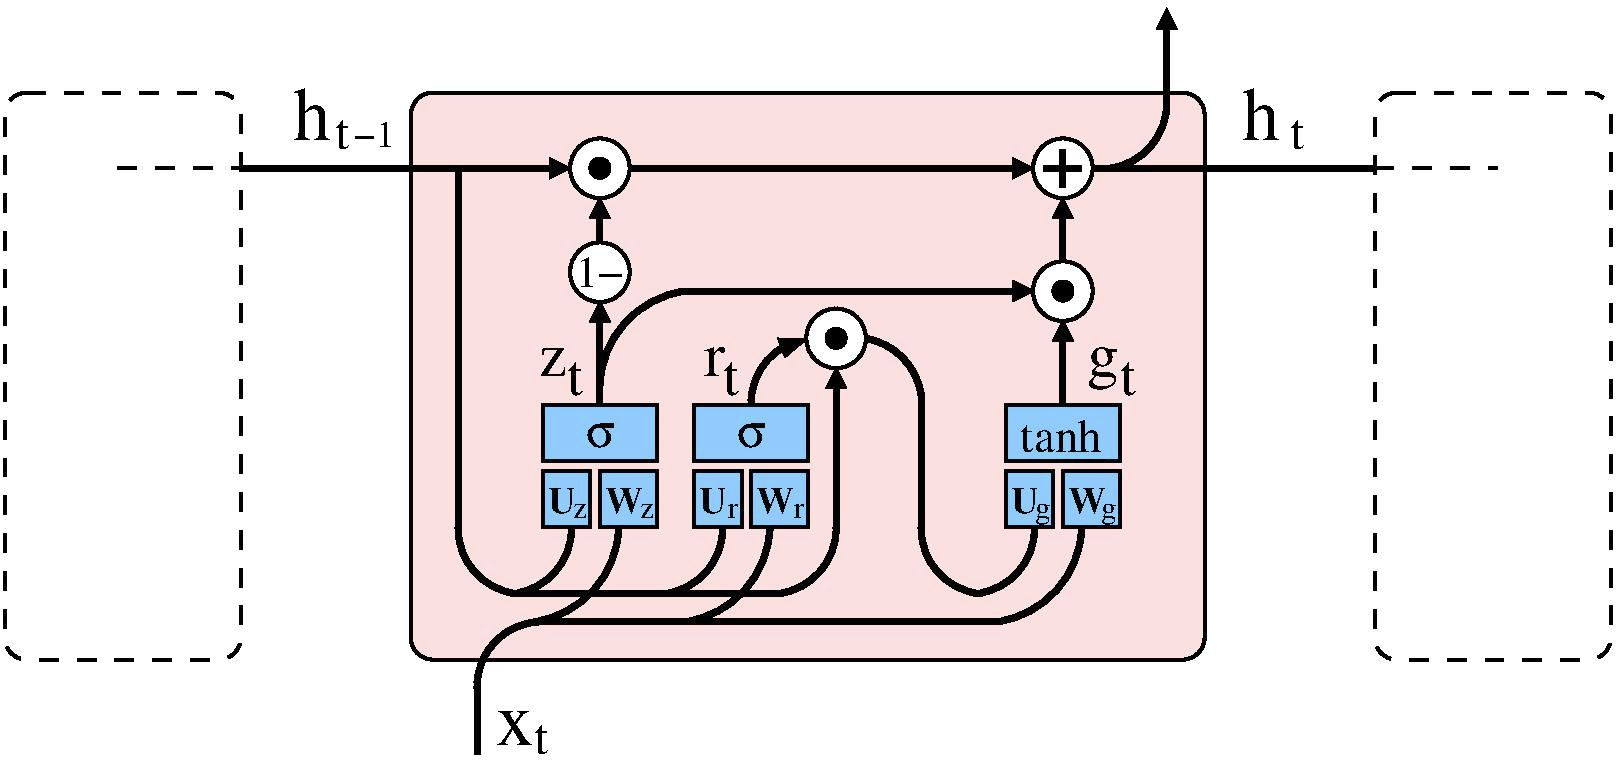
\includegraphics[height=6,width=12]{../out/images/gated-recurrent-unit}
    \caption[gated recurrent unit]{gated recurrent unit}
    \label{fig: gated recurrent unit}
\end{figure}

The Gated Recurrent Unit (GRU) is similar to LSTM but has only two gates
instead of three.
Its update equations are as follows:

\textbf{Gates}

\begin{gather*}
    z_t = \sigma (U_{z}h_{t-1} + W_{z}X_t + b_z)\\
    r_t = \sigma (U_g(r_t \odot h_{t-1}) + W_g X_{t} + b_g)\\
\end{gather*}

\textbf{Candidate Activation}

\textbf{Output}

\subsection{further reading}\label{subsec:further-reading}

Fahlman, S. E. (1991). \href{https://citeseerx.ist.psu.edu/viewdoc/download?doi=10.1.1.52.7163&rep=rep1&type=pdf}{The recurrent cascade-correlation architecture} (Technical Report CMU-CS-91-100). Carnegie-Mellon University, Department of Computer Science.

Hochreiter, S., and Schmidhuber, J., 1997. \href{http://citeseerx.ist.psu.edu/viewdoc/download?doi=10.1.1.676.4320&rep=rep1&type=pdf}{Long short-term memory}. Neural Computation, 9(8), 1735-1780.

Two excellent web resources for LSTM:
- \href{http://colah.github.io/posts/2015-08-Understanding-LSTMs/}{Understanding LSTM Networks} (Colah, 2015. Github)
- \href{http://christianherta.de/lehre/dataScience/machineLearning/neuralNetworks/LSTM.php}{LSTM (Long Short Term Memory} (Huerta, n.d. christianherta.de)
- \href{https://www.deep-teaching.org/notebooks/sequence-learning/exercise-pytorch-char-rnn-reber-grammar}{LaTeX-Tutorial}Use of Reber Grammar


\end{document}